%!TEX root = ../thesis.tex
%*******************************************************************************
%****************************** Third Chapter **********************************
%*******************************************************************************
\chapter{Introduction to Quantum Annealing} \label{chapter: QA}

% **************************** Define Graphics Path **************************
\ifpdf
    \graphicspath{{Chapter3/Figs/Raster/}{Chapter3/Figs/PDF/}{Chapter3/Figs/}}
\else
    \graphicspath{{Chapter3/Figs/Vector/}{Chapter3/Figs/}}
\fi
Quantum computing represents a revolutionary approach to computational technology, utilizing principles of quantum mechanics like superposition and entanglement to perform operations far beyond the capabilities of classical computers. This chapter introduces quantum computing, emphasizing its potential to solve complex, intractable problems for traditional systems.

Furthermore, the chapter explores quantum annealing (QA), a promising quantum computing approach. It explains QA problem formulation and annealing algorithms, particularly highlighting the use of D-Wave systems for practical quantum annealing applications. %This discussion sets the stage for subsequent chapters that will delve into the integration of quantum computing technologies, like QA, in wireless communication, a domain poised to benefit significantly from the enhanced computational power of quantum technologies.
\section{Computational Complexity}

Computational complexity theory, a branch of theoretical computer science, classifies problems into different classes based on the computational effort required to solve them, primarily focusing on time and space. Key complexity classes for combinatorial optimization problems As shown in \autoref{fig:NP} include P, NP, NP-complete, and NP-hard. The P (Polynomial) class encompasses decision problems solvable efficiently with deterministic polynomial-time algorithms. Conversely, the NP (Non-deterministic Polynomial) class includes decision problems that, although challenging to solve in polynomial time, have solutions that are verifiable within polynomial time.

NP-complete problems represent the most challenging problems within the NP class, being both verifiable in polynomial time and reducible from any other NP problem in polynomial time. NP-hard problems, while as challenging as NP-complete problems, may not be decision problems and might not have verifiable solutions in polynomial time \cite{Nielsen2002}.
\begin{figure}[H]
    \centering
    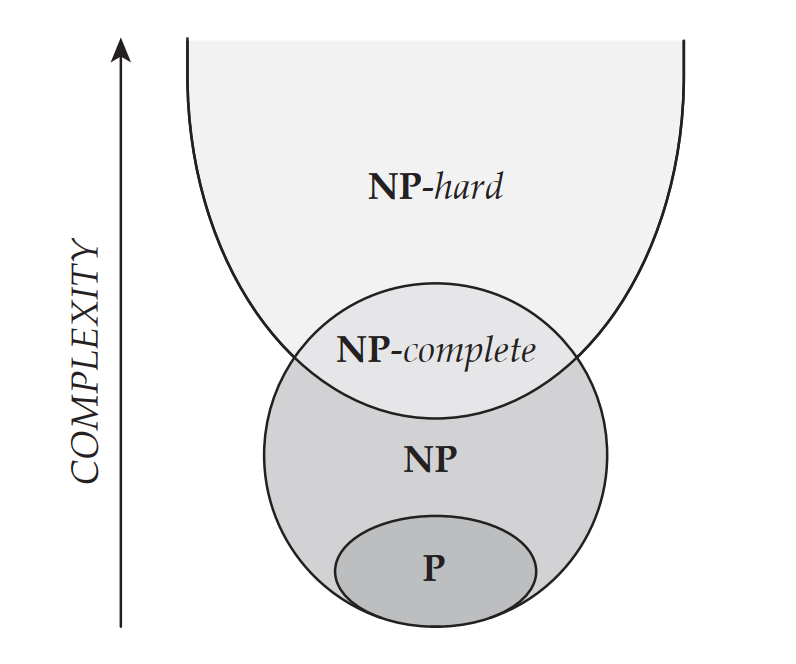
\includegraphics[width=0.5\linewidth]{NP.png}
    \caption{Sketch representing the relation between the different complexity classes P, NP,
NP-complete, and NP-hard.}
    \label{fig:NP}
\end{figure}

Combinatorial optimization problems, which require finding an optimal arrangement of a finite set of objects to minimize or maximize a cost function, are typically NP-hard. Such problems pervade fields like artificial intelligence and machine learning.

Quantum computing holds potential for addressing some NP-hard problems more effectively than classical computing by utilizing quantum phenomena such as superposition and entanglement. These capabilities allow quantum algorithms to explore solution spaces more comprehensively, potentially accelerating the convergence to optimal or near-optimal solutions \cite{Benenti2004}. 
%Quantum annealing, an optimization algorithm inspired by metallurgical annealing, uses qubits in quantum annealers, such as those developed by D-Wave Systems, to represent variables and guide the system toward lower-energy states indicative of optimal solutions.

This project utilizes quantum annealing to tackle the Maximum Likelihood (ML) detection problem in communication systems—an NP-hard problem. By representing the ML as a combinatorial optimization problem and solving it using a quantum annealer, this work aims to demonstrate how quantum computing can significantly enhance communication system performance and efficiency. As quantum technology progresses, it is anticipated to complement classical computing in resolving complex optimization challenges across various domains, including communication systems.

\section{Fundamentals of Quantum Computation}

Quantum computation offers a significant advance over traditional computing by employing quantum mechanics' distinctive properties—superposition, entanglement, and quantum tunneling. Additionally,The inherent parallelism of quantum information processing
intimated in \autoref{fig:QAvsPC} equips quantum computers with immense
computational power.  Unlike conventional computers that operate with bits represented solely by 0s or 1s, quantum computers utilize qubits. These qubits can represent multiple states simultaneously due to superposition, enhanced by the interconnectedness of states via entanglement and the non-classical movement of quantum tunneling. This capacity allows quantum computers to process complex data configurations and solve problems that are currently infeasible for classical systems.
\begin{figure}[H]
    \centering
    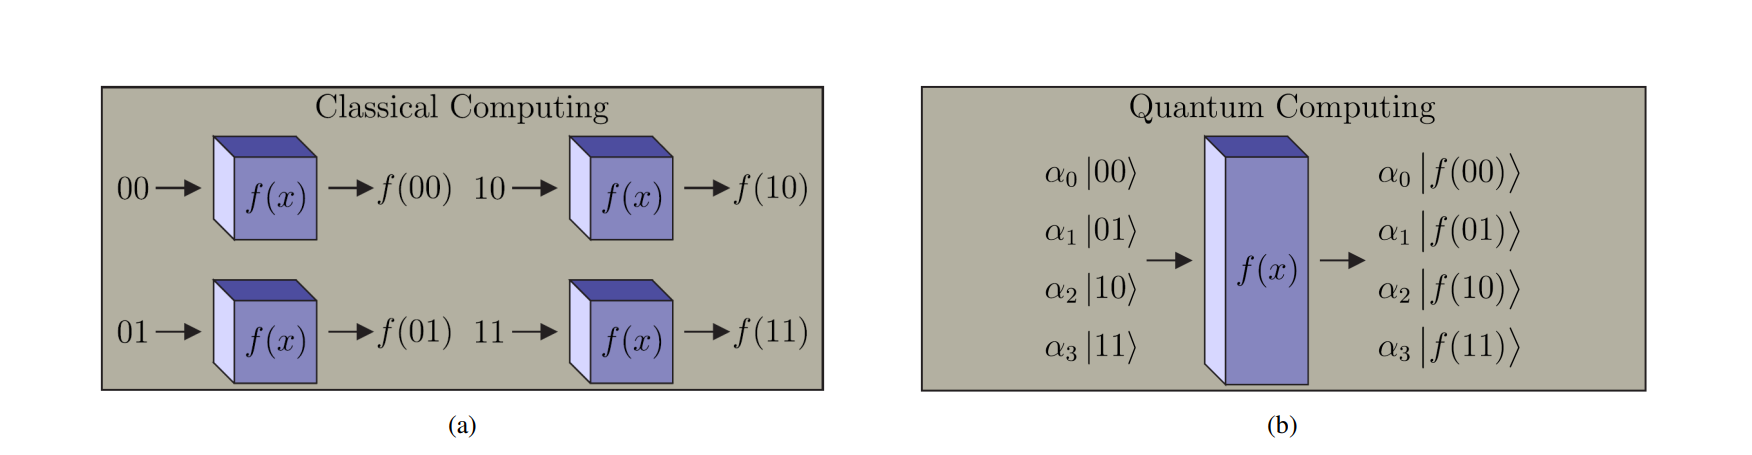
\includegraphics[width=1\linewidth]{Untitled.png}
    \caption[The comparison of classical and quantum computation.]{The comparison of classical and quantum computation \cite{Benenti2004}.}
    \label{fig:QAvsPC}
\end{figure}


\subsection{Quantum Systems and States}

In quantum mechanics, the behavior of quantum systems is governed by Schrödinger's equation, the quantum analogue of Newton's second law in classical mechanics. This fundamental equation describes how the wavefunction of a physical system evolves over time, dictated by the Hamiltonian, a Hermitian operator that determines the system's discrete energy levels. Schrödinger's equation is given by:
\begin{equation}
    i \,  \, \hbar \frac{\partial}{\partial t} |\psi(t)\rangle = \hat{H} |\psi(t)\rangle
\end{equation}
where \(\hbar\) is the reduced Planck's constant, \(i\) is the imaginary unit, \(|\psi(t)\rangle\) represents the state vector of the system at time \(t\), and \(\hat{H}\) is the Hamiltonian operator \cite{Griffiths2018}.

The energy levels of a quantum system are determined by the eigenvalues of the Hamiltonian. Since the Hamiltonian is \textit{Hermitian}, all eigenvalues are real numbers, making these energy levels physically observable. The smallest eigenvalue corresponds to the ground state energy, the second smallest to the first excited state, and so forth. Quantum systems exist only in these discrete energy states—either the ground state or an excited state—but not in between, in other words are "quantized." This concept underlies the term \textit{quantum}, derived from \textit{quanta}.

Quantum states are represented as vectors in a complex vector space known as Hilbert space. In Dirac notation, a quantum state is denoted as \(|\alpha\rangle\), where \(\alpha\) includes complex numbers that are probability amplitudes.

\textbf{Superposition} is a distinguishing feature of quantum systems is their ability to exist in states of superposition. Unlike classical systems, which are confined to a single state at any given time, quantum systems can simultaneously inhabit multiple states. For instance, a state \(|\phi\rangle\) might be a superposition of two basis states \(|a\rangle\) and \(|b\rangle\), expressed as:
\begin{equation}
    |\phi\rangle = c_a |a\rangle + c_b |b\rangle
\end{equation}
where \(c_a\) and \(c_b\) are complex coefficients, and the probabilities of finding the system in either state upon measurement are \(|c_a|^2\) and \(|c_b|^2\) respectively.

\textbf{Entanglement} is another pivotal phenomenon, which occurs when pairs or groups of particles interact such that the state of one particle cannot be described independently of the others, regardless of the distance between them. A classic example is a two-particle system in a Bell state:
\begin{equation}
    |\psi\rangle = \frac{1}{\sqrt{2}} (|aa\rangle + |bb\rangle)
\end{equation}
In this state, if one particle is measured and found in state \(|a\rangle\) or \(|b\rangle\), the other particle will instantaneously be found in the same state, demonstrating quantum non-locality. This effect, where entangled particles affect each other instantaneously over any distance without direct physical connection, has no equivalent in classical physics and illustrates the unique, interconnected nature of quantum systems \cite{Griffiths2018}.
\subsection{The Qubit}

The qubit is the fundamental unit of quantum information, analogous to the classical bit in conventional computing. However, unlike classical bits, which can only exist in one of two states (0 or 1), a qubit can exist in a superposition of these states. The quantum state of a qubit, represented in an orthogonal basis commonly referred to as the computational basis \(\{|0\rangle, |1\rangle\}\), is expressed as:
\begin{equation}
    |q\rangle = \alpha|0\rangle + \beta|1\rangle
\end{equation}
where \(\alpha\) and \(\beta\) are complex numbers (\(\alpha, \beta \in \mathbb{C}\)) representing the amplitudes of the qubit state on the computational basis, and the condition \(\|\alpha\|^2 + \|\beta\|^2 = 1\) ensures the normalization of the state.

In the special cases where \(\alpha = 0\) and \(\beta = 1\), the qubit state simplifies to \(|q\rangle = |1\rangle\), corresponding to the classical bit value 1. Conversely, when \(\alpha = 1\) and \(\beta = 0\), the state becomes \(|q\rangle = |0\rangle\), analogous to the classical bit value 0. For the case of equal superposition, where \(\alpha = \beta = 1/\sqrt{2}\), the qubit is in the state:
\begin{equation}
    |q\rangle = \frac{1}{\sqrt{2}}(|0\rangle + |1\rangle)
\end{equation}
This state does not favor either of the orthogonal states \(|0\rangle\) or \(|1\rangle\), and is widely utilized in quantum algorithms due to its symmetric properties \cite{Nielsen2002}.

Geometrically, the state of a qubit can be depicted using a 2-D or 3-D representation. For real-valued amplitudes, the qubit state simplifies to:
\begin{equation}
    |q\rangle = \cos(\theta)|0\rangle + \sin(\theta)|1\rangle
\end{equation}
and can be visualized on a 2-D plane. For complex-valued amplitudes, a more comprehensive representation on the 3-D Bloch sphere is used shown in \textbf{\autoref{fig:qubit}}, where the qubit state is expressed as:

\begin{equation}
    |q\rangle = \cos(\frac{\theta}{2})|0\rangle + e^{i\phi}\sin(\frac{\theta}{2})|1\rangle
\end{equation}
\begin{figure}[H]
    \centering
    \includegraphics[width=0.4\linewidth]{qubit.png}
    \caption[Qubit represented by Bloch sphere.]{The Bloch sphere is a 3-D geometrical representation of the pure state space of a two-level quantum mechanical system (qubit), named after the physicist Felix Bloch \cite{Nielsen2002}.}
    \label{fig:qubit}
\end{figure}
Measuring the state of a qubit collapses the superposition to one of the orthogonal states \(|0\rangle\) or \(|1\rangle\), with probabilities \(\|\alpha\|^2\) and \(\|\beta\|^2\) respectively. This process, akin to a quantum-to-classical conversion, provides critical insights into the quantum system's state \cite{Benenti2004}.
Post-measurement, the quantum state of the system collapses irreversibly to the observed state. For example, if a measurement of a qubit in an equal superposition state yields \(|1\rangle\), the post-measurement state of the qubit becomes \(|q'\rangle = |1\rangle\).

Moreover, qubits can exhibit quantum \textbf{entanglement}, a property allowing multiple qubits to demonstrate correlations exceeding those possible in classical systems. Consider two qubits in the entangled Bell state:
\begin{equation}
    \frac{1}{\sqrt{2}}(|00\rangle + |11\rangle)
\end{equation}
Here, if one qubit is measured and found to be \(|0\rangle\) or \(|1\rangle\), the state of the other qubit is instantaneously known, regardless of the distance separating them. This perfect correlation, demonstrating quantum non-locality, is one of the many counterintuitive aspects of quantum physics \cite{QAMUD}.

To physically implement qubits, any two-level quantum-mechanical system can be used. Multilevel systems can be used as well, if they possess two states that can be effectively decoupled from the rest (e.g., the ground state and first excited state of a nonlinear oscillator). Several physical implementations that approximate two-level systems to various degrees have been successfully realized, most common are \textit{trapped ions, quantum dot} and \textit{Josephson junction} \cite{Preskill2018}.



\subsection{Models of Quantum Computation}

Quantum computation primarily encompasses two models: \textbf{gate-based quantum computing} and \textbf{adiabatic quantum computation} (\textbf{AQC}). Current quantum computers, referred to as \textbf{Noisy Intermediate-Scale Quantum} (\textbf{NISQ}) devices, include both gate models and quantum annealers. These NISQ devices comprise hundreds of noisy qubits which perform operations with limited precision and coherence \cite{Preskill2018}.

The \textit{gate model} of quantum computing uses \textit{unitary gates} to manipulate qubits in a manner analogous to digital computing, with operations based on quantum mechanical properties. This model includes algorithms like the \textbf{Quantum Approximate Optimization Algorithm} (QAOA), which aims to optimize computational solutions, constrained by the current qubit number.

\textbf{Adiabatic quantum computation}, or quantum annealing, operates similarly to analog computing. It starts from a simple Hamiltonian's ground state and evolves towards a complex final Hamiltonian to solve optimization problems through gradual parameter adjustments \cite{Farhi2001}.

NISQ devices are influenced by environmental noise sources such as thermal baths and electromagnetic cross-talk, affecting their operational efficiency. Future advancements are expected to enhance the performance significantly.



\section{Quantum Annealing}

Quantum annealing (QA) is a heuristic optimization algorithm that leverages quantum mechanics to solve complex combinatorial optimization problems. Analogous to the metallurgical process of \textit{annealing}, which involves heating and then slowly cooling to remove defects, quantum annealing utilizes quantum-mechanical fluctuations, notably \textit{quantum tunneling}, to navigate the solution space. %Quantum tunneling allows a system to transition through potential energy barriers even when it does not possess sufficient classical energy to overcome these barriers. This property is critical in quantum annealing, as it enables the exploration and escape from local minima in pursuit of the global minimum of an objective function across a set of candidate solutions.
The concept of quantum annealing was initially proposed in 1988 and has since been developed into a robust computational strategy that manipulates quantum fluctuations to resolve optimization challenges that are impractical for classical computers \cite{QAKadowaki1998QuantumAI}.
%Quantum annealing has become particularly relevant with the advent of small- and intermediate-scale quantum processors, such as those developed by \textit{D-Wave Systems}, which allow for programmable quantum annealing in various research and industrial applications. These processors are used to tackle problems characterized by many local minima, such as finding the ground state of a spin glass or optimizing routes in the traveling salesman problem. 
\subsection{Adiabatic Quantum Computation Model}

Quantum Annealing relies on the adiabatic quantum computation (AQC) which is a scheme of quantum computation.In this scheme a physical system is initially
prepared in its known lowest energy configuration, or ground state. The computation
involves gradually deforming the system’s Hamiltonian, very slowly, to assure that the
system remains in its ground state throughout the evolution process. One designs the
evolution of the Hamiltonian such that the ground state of the final Hamiltonian is the
solution to the optimization problem. AQC is based on the adiabatic theorem that states \cite{Tanaka2017QuantumSG}:
\textit{“A physical system remains in its instantaneous eigenstate if a given perturbation is
acting on it slowly enough and if there is a gap between the eigenvalues and the rest of the
Hamiltonian spectrum.”}. 

The Hamiltonian is therefore time dependent $H = H(t)$. The initial Hamiltonian $H_0 = H(0)$ and its lowest energy eigenvector should be easy to construct. We assume the final Hamiltonian $H_T$ is also easy to construct, however its ground state which is the solution to our optimization problem could be exponentially hard to find with a classical algorithm. The Hamiltonian of the AQC is therefore \cite{berwald2018mathematics}:
\begin{equation}
H(t) = \left(1 - \frac{t}{\tau}\right)H_0 + \frac{t}{\tau} H_T = (1 - s)H_0 + sH_T,
\end{equation}
where $\tau$ is the \textit{adiabatic time scale}, and $t$ goes from 0 to $\tau$. The complexity of the adiabatic algorithm is manifested in the time it takes to evolve the computer from its initial to its final state. It can be shown that the adiabatic approximation is valid when the annealing time satisfies \cite{Tanaka2017QuantumSG}:
\begin{equation}
\tau \gg \frac{\max_{0 \leq s \leq 1}\left|\frac{1}{s}\frac{dH(s)}{ds} \frac{1}{\langle 0(s) | 0(s) \rangle}\right|}{\min_{0 \leq s \leq 1}\Delta_{10}(s)^2},
\end{equation}
where $|i(s) \rangle$ for $i = 0, 1$ are the ground and first excited states of $H(s)$, and $\Delta_{10}(s)$ is their energy difference.
Given a time-dependent Hamiltonian, we can write:
\begin{equation}
H | \psi_n(t) \rangle = E_n(t) | \psi_n(t) \rangle,
\end{equation}
where $| \psi_n(t) \rangle$ (resp. $E_n(t)$) is the $n$-th eigenvector (resp. eigenvalue) \cite{Tanaka2017QuantumSG}. The general solution to the Schrödinger equation can be written as:
\begin{equation}
| \psi(t) \rangle = \sum_n c_n(t) | \psi_n(t) \rangle e^{i \theta_n(t)},
\end{equation}
where $\theta_n(t)$ is known as the dynamic phase. Using the Schrödinger equation, one can verify that:
\begin{equation}
c_n(t) = -c_n(t) \langle \psi_n(t) | \psi_n(t) \rangle - \sum_{m \neq n} c_m(t) \frac{\langle \psi_n(t) | H | \psi_m(t) \rangle}{E_m - E_n} e^{i(\theta_m - \theta_n)}.
\end{equation}
Now, to ensure that the evolution of the $n$-th eigenstate remains as the $n$-th eigenstate, we have to reduce the amplitude:
\begin{equation}
\frac{\langle \psi_n(t) | H | \psi_m(t) \rangle}{E_m - E_n}.
\end{equation}
This can be done by varying H(t) very slowly with respect to ${E_m - E_n}$, which posits that a quantum system will remain in its ground state throughout a process if the Hamiltonian governing it changes sufficiently slowly. This condition hinges critically on the minimum energy gap between the ground state and the first excited state, often referred to as the \textit{minimum gap} \cite{QAKadowaki1998QuantumAI}.
\subsection{Quantum Annealing Algorithm}

%In quantum mechanics, the Hamiltonian is an operator that defines the total energy of a system at any given state, analogous to its counterpart in classical mechanics. It maps specific states, known as eigenstates, to their corresponding energy levels, termed eigenenergies. The system's state is fully described by its wavefunction, with the Hamiltonian dictating the evolution of this wavefunction \cite{Yarkoni2022}.
The quantum algorithm is started by preparing the system in the ground state of a Hamiltonian,
which is known and easy to prepare, denoted as $H_i$ (also known as the initial Hamiltonian). Then,
the system is slowly changed such that the contribution of $H_i$ is slowly reduced while the magnitude
of a final (also known as target) Hamiltonian, denoted $H_f$, is increased (using time parameter $t$)  \cite{Tanaka2017QuantumSG}:
\begin{equation}
H(t) = A(t) H_i + B(t) H_f
\end{equation}
The time $t \in [0, T_a]$, where \( A(t) \) and \( B(t) \) are monotonic functions that manage the annealing schedule, starting with \( A(0) = 1 \) and \( B(0) = 0 \), transitioning to \( A(T_a) = 0 \) and \( B(T_a) = 1 \) by the end of the annealing process at time \( T_a \).

The gradual transition from $H_i$ to $H_f$ induces an evolution from the initial (ground) state $|\psi(t = 0)\rangle$ to the ground state $|\psi(t = T_a)\rangle$ of the final Hamiltonian $H_f$, where $|\psi(t)\rangle$ represents the time-dependent wavefunction in the Dirac bra-ket notation. Typically, a transverse field in x-direction is used as the initial Hamiltonian,
\begin{equation}
H_i = \sum_{i \in V} \sigma^x_i,
\end{equation}
where $\sigma^x_i$ is the x-Pauli matrix acting on the i-th qubit:
\begin{equation}
\sigma^x = \begin{pmatrix} 0 & 1 \\ 1 & 0 \end{pmatrix}, \quad
\sigma^z = \begin{pmatrix} 1 & 0 \\ 0 & -1 \end{pmatrix}.
\end{equation}
The Pauli opertator $\sigma^x$ induces flips of the $\sigma^z$-basis states as $\sigma^x|\pm\rangle = |\mp\rangle$ and its eigenstates are $|x\pm\rangle = \frac{1}{\sqrt{2}}(|+\rangle + |-\rangle)$, which are equal amplitude superposition of the $\sigma^z$ eigenstates. Thus, initially, the system is prepared in the ground state to $H_i$, which is given by $|\psi(t = 0)\rangle = |x-,\cdots,x-\rangle$. The final Hamiltonian is represented by  \cite{QAKadowaki1998QuantumAI}:
\begin{equation}
H_f = \sum_{i \in V} h_i \sigma^z_i + \sum_{(i,j) \in E} J_{ij} \sigma^z_i \sigma^z_j,
\end{equation}
Here, $V$ is the set of vertices of the graph $G(V,E)$ representing the lattice sites where qubits are located, $E$ the set of edges of the graph connecting the qubits, $J_{ij} = J_{ji}$ are the symmetric interaction strength of the qubits $i$ and $j$ connected by an edge and $h_i$ is the on-site energy (local field) of qubit $i$. For any given time $t$, the Hamiltonian $H(t)$ of Eq. (3.15) is the transverse-field Ising Hamiltonian. As the magnitude of $H_i$ decreases, the quantum dynamics of the qubits slows down until at $t = T_a$ we obtain a purely classical system, where the final states of the qubits are measured. The classical Ising model is obtained by replacing the quantum $\sigma^z$ Pauli operators by classical spin variables  \(s_i \in \{+1, -1\}\) (all other terms are the same as in Eq. (3.18)):
\begin{equation}
H_{\text{Ising}} = \sum_{i \in V} h_i s_i + \sum_{(i,j) \in E} J_{ij} s_i s_j.
\end{equation}

\begin{figure}
    \centering
    \includegraphics[width=0.75\linewidth]{schedule.png}
    \caption{A typical annealing schedule. Scales are arbitrary; energy is measured in GHz. The parameter \textbf{\textit{s}}
evolves from 0 to 1, on the scale of microseconds \cite{berwald2018mathematics}.}
    \label{fig:enter-label}
\end{figure}

Figure 3.4 shows two anneal schedule signals as a function of $s$, Specifically, $s$ is defined as $s = \frac{t}{\tau}$. where $A(s)$ represents the transverse energy
that controls the strength of the quantum fluctuations (i.e., quantum-coherent exploration of
the search space), while $B(s)$ is the energy that is meant to correlate these fluctuations to
the problem energy function (Eq. 3.18).

In the standard QA (called \textit{Forward Annealing} or FA), the system initially applies strong
quantum fluctuations and prepares a quantum superposition state that holds every possible
configuration information (i.e., $A(s) \gg B(s)$ at $s = 0$), and then drives the changes until the
effect of the initial superposition $H_i$ diminishes (i.e., $A(s) \ll B(s)$ at $s = 1$).\footnote{A state at s = 0 indicates a fully quantum state, while a state at s = 1 indicates a fully classical state.} During the anneal
duration (user parameter range: $T_a \in [0.5, 2000 \, \mu s]$), $s$ increases incrementally from 0 to
1, hoping that the adiabatic nature of the thermodynamics will lead to a
low-energy state (a ground state in ideal cases), despite the noisy, imperfect implementation
of the current hardware.

At the end of the anneal protocol, the Pauli $\sigma$ operators in $H_i$ and $H_f$ can be identified to spin
values, and the system can interpret the result as a classical spin state/configuration, being
a \textit{sample}. Since QA is a probabilistic technique, the end result is non-deterministic. Thus,
multiple runs of the solver ($N_a$ or anneal counts) are typically applied, which will lead to
$N_a$ configuration samples. Among them, the best sample $s$ (i.e., $\min E(s)$) is filtered as a
final optimization solution \cite{Kim2019}.



\subsection{Problem Formulation for Quantum Annealing: QUBO and Ising Model}

Quantum Annealing (QA) requires the problem of interest to be defined as an objective function, typically a quadratic polynomial of binary variables. This objective function is then expressed in one of two equivalent forms: the Ising model or the Quadratic Unconstrained Binary Optimization (QUBO) model, in which can be used to construct the Hamiltonian.

\paragraph{Ising Model Formulation}
In the Ising model, defined in Eq.(3.19), can be rewritten in optimization form \cite{QAKadowaki1998QuantumAI}:
\begin{equation}
s_1, \dots, s_{N_v} = \arg \min_{s_1, \dots, s_{N_v}} \left( \sum_{i<j}^{N_v} J_{ij}s_i s_j + \sum_{i=1}^{N_v} h_i s_i \right) \label{equation: ising}
\end{equation}
where $s_i \in \{-1, 1\}$ are the spin variables and $h_i$, $J_{ij}$ contain the Ising model's coefficients corresponding to the biases and coupling strengths, respectively, and \textit{$\mathbf{s}$} is a minimum energy Ising spin configuration vector.

\paragraph{QUBO Formulation}
The QUBO model uses classical binary bits \(q_i \in \{0, 1\}\) to represent the problem \cite{Tanaka2017QuantumSG}:
\begin{equation}
q_1, \dots, q_{N_v} = \underset{q_1, \dots, q_{N_v}}{\arg \min} \left( \sum_{i \leq j}^{N_v} Q_{i,j}q_i q_j \right) 
\end{equation}
where \(Q_{ij}\) includes both \textit{linear terms} (on the diagonal) and \textit{quadratic terms} (off-diagonal), where $\textbf{Q} \in \mathbb{R}^{N_v \times N_v}$ is upper triangular. The off-diagonal matrix elements $Q_{ij}$ ($i \neq j$) correspond to $J_{ij}$ in \autoref{equation: ising}, and the diagonal elements correspond to $h_i$.
\[
\textbf{Q }= \begin{bmatrix}
Q_{11} & Q_{12} & \cdots & Q_{1N_v} \\
0 & Q_{22} & \cdots & Q_{2N_v} \\
\vdots & \vdots & \ddots & \vdots \\
0 & 0 & \cdots & Q_{N_v N_v} \tag{3.13b}
\end{bmatrix}
\]

The two forms are equivalent, their solutions related by:
\begin{equation}
q_i \leftrightarrow \frac{1}{2}(s_i + 1), 
\end{equation}

leading to 
\begin{equation}
J_{ij} \leftrightarrow \frac{1}{4}Q_{ij} \quad \text{and} \quad h_i \leftrightarrow \frac{1}{2}Q_{ii} + \frac{1}{4} \sum_{k=1}^{i-1} Q_{ki} + \frac{1}{4} \sum_{k=i+1}^{N_v} Q_{ik}.
\end{equation}

 \autoref{table:quboising} compares the terms associated with each model and their equivalence on the physical QPU.
\begin{table}[h]
    \centering
    \caption{Comparison of problem expressions and their terms in various contexts.}
    \label{table:quboising}
    \begin{tabular}{@{}ccccc@{}}
        \toprule
        \multirow{2}{*}{Problem Expression} & \multicolumn{4}{c}{Terms} \\ 
        \cmidrule(lr){2-5} % Line under the "Terms"
        & Linear coefficient & Quadratic coefficient & Variable & States \\
        \midrule
        QUBO (scalar) & \(a_i\) & \(b_{ij}\) & \(q_i\) & \(\{0, 1\}\) \\
        QUBO (matrix) & \(Q_{ii}\) & \(Q_{ij}\) & \(x_i\) & \(\{0, 1\}\) \\
        Ising & \(h_i\) & \(J_{ij}\) & \(s_i\) & \(\{-1, 1\}\) \\
        Graph & Node Weight & Edge Strength & Node & - \\
        QPU & Qubit Bias & Coupling Strength & Qubit State & \(\{\text{Spin Up}, \text{Spin Down}\}\) \\
        \bottomrule
    \end{tabular}
\end{table}

\section{D-Wave Implementation of Quantum Annealing }

\textbf{D-Wave Systems}, based in Canada, leads the field in developing and commercializing quantum computers through the method of quantum annealing. 
The company's core technology, the Quantum Processing Unit (QPU), employs qubits designed to identify low-energy states that correspond to optimal solutions, thus efficiently solving complex optimization challenges. Since introducing the first commercial quantum annealer, the D-Wave One, in 2011, equipped with a 128-qubit processor, D-Wave has consistently advanced the capabilities of its technology \cite{dwavearticle}.



\subsection{Hardware Architecture of D-Wave Quantum Annealing System}
The core of an annealing QPU is an array of qubits, each of which realizes a simple two-level quantum system. D-Wave Systems utilize superconducting flux qubits to build their QPU.

The superconducting flux qubits in D-Wave's quantum annealers are niobium-based \textit{radio-frequency SQUIDs} (\textbf{rf-SQUIDs}) that utilize superconducting current loops interrupted by two \textit{Josephson junctions}. These junctions are controlled by variable magnetic fluxes as illustrated in \autoref{fig:rf}. Each qubit is a double-ring shaped niobium structure with two Josephson junctions that regulate the flow of current within the ring. The direction of the current, which can be clockwise, counterclockwise, or a superposition of both when the qubit is in a quantum superposition state, determines the magnetic forces represented as spin-up, spin-down, or a combination of both \cite{dwavearticle}.

\begin{figure}[H]
    \centering
    \includegraphics[width=0.5\linewidth]{rfsquid.png}
    \caption{Each qubit is a loop of niobium controlled by Josephson junctions and biases represented by $\phi$ in this diagram \cite{dwavearticle}.}
    \label{fig:rf}
\end{figure}

\textbf{Couplers}, which connect pairs of qubits, consist of simpler niobium loops with less control circuitry compared to the qubits. Both qubits and couplers are etched onto \textit{silicon wafer circuits} with four niobium layers separated by insulation layers. Although this technology is robust against various types of noise, it remains sensitive to electromagnetic interference, necessitating that the quantum processing unit (QPU) operates in a shielded chamber with a temperature below 15 mK, a magnetic field 50,000 times weaker than Earth's, and an atmospheric pressure 10 billion times lower than the ambient environment \cite{dwavearticle}.



\subsection{Topology of D-Wave's QPU and Embedding}

The quantum chips in D-Wave systems use a unique topology to lay out their qubits, defining the physical connections between qubits and their couplers, which in turn fundamentally influences how algorithms are implemented and executed on these systems. Two of the most notable topologies developed by D-Wave are Chimera and Pegasus. Figure 3.6 illustrates the unit cell of each topology.

\paragraph{Chimera Topology}
The Chimera topology, utilized in earlier D-Wave systems, features a two-dimensional lattice of unit cells. Each cell is a complete bipartite graph \(K_{4,4}\), allowing each qubit in one partition to connect to all qubits in the opposing partition. This setup facilitates a connectivity of six for each qubit, supporting a variety of optimization problems but with limitations due to its relatively sparse connectivity.
\begin{figure}[H]
    \centering
    \includegraphics[width=0.8\linewidth]{topology.png}
    \caption[Unit cells and their connections of currently available D-Wave hardware topology.]{Unit cells and their connections of currently available D-Wave hardware topology. The older QPU (D-Wave 2000Q) uses a less connected Chimera \(C_{16}\) architecture (a) with degree 6, while the new Advantage System uses the denser Pegasus \(P_{16}\) architecture with degree of 15 (b). Here, only \(C_2\) and a \(P_2\) graphs are depicted \cite{dwavetop}.}
    \label{fig:enter-label}
\end{figure}
\paragraph{Pegasus Topology}
Advancing from Chimera, the Pegasus topology, introduced with the D-Wave Advantage series, significantly increases qubit connectivity. Each qubit in Pegasus is connected to fifteen others, enhancing the system's ability to handle more complex optimization challenges. This topology is structured into a more intricate mesh of qubits, enabling denser graph structures and higher problem-solving capabilities.

Despite the sophisticated designs, not all qubits and couplers may be operational due to manufacturing imperfections or calibration issues, with the hardware yield typically around 97\%. The working graph, representing the functional part of the full hardware graph, directly impacts the size and complexity of problems that the QPU can effectively address \cite{QAembeddingwirless}.

\paragraph{The Need for Embedding}
Much like a classical computer converts high-level, abstract, and human-readable languages to machine instructions, QUBO's must be converted to a \textit{quantum machine instruction (QMI)} that will run on the quantum computer. There are numerous steps in this process, one of which, \textit{embedding}. In many cases, QUBO models have high connectivity, which makes them challenging to map directly onto QPU hardware topologies. It is convenient to view the problem Hamiltonian, \(H_P\), as a weighted graph. Define \(G = (V, E)\), where the node set \cite{berwald2018mathematics}:
\begin{equation}
    V = \{(u_1, \alpha_1), \ldots, (u_n, \alpha_n) \mid \alpha_i = h_i\}
\end{equation}


is composed of nodes \(u_i\) that are in direct correspondence with each binary variable \(x_i\), where \(x = (x_1, \ldots, x_n) \in \mathbb{B}^n\). Each node is weighted by the bias \( \alpha_i = h_i\). Similarly, the edge set is composed of weighted edges defined by the coupling terms in \(H_P\), so that
\begin{equation}
    E = \{(u_i, v_j, \omega_{i,j}) \mid u_i, v_j \in V \text{ and } \omega_{i,j} = J_{i,j}, J_{i,j} \neq 0\}.
\end{equation}

This definition of \(E\) encodes the variable coupling in \(H_P\).

The graph \(G\) must be embedded onto the hardware to solve \(H_P\). Embedding the \textit{logical graph}, \(G\), onto the \textit{hardware graph}, \(C\), amounts to finding a \textit{minor embedding}. A \textit{minor} of a graph \(H\) is a subgraph of \(H\) obtained by contracting or deleting edges, or omitting isolated vertices. A minor embedding is a function that maps the vertices of \(G\) to the power set of the vertices of \(C\),
\[
\psi: V_G \rightarrow 2^{V_C},
\]
such that for each \(u \in V_G\), the image \(\psi(u) \in V_C\) is connected. These connected components within the hardware graph are termed \textit{chains}. Embeddings for which \(\psi(u)\) is a singleton for all \(u\) are called \textit{native embeddings} \cite{dwaveembed}. Lastly, there exists an edge between \(\psi(u)\) and \(\psi(v)\) whenever \(u\) and \(v\) are adjacent in the logical graph. The map \(\psi\) is the minor embedding we seek. Figure 3.7 outlines examples of minor embedding.
\begin{figure}[H]
    \centering
    \includegraphics[width=0.84\linewidth]{embedding.png}
    \caption[Examples of minor embedding.]{ Examples of minor embedding into the $(1, 1, 4)$-Chimera of the complete graphs $K_3$, $K_4$, and $K_5$.\footnotemark \protect}
    \label{fig:embedding}
\end{figure}
\footnotetext{The numbers and colors of the vertices in the graph are the same as in the minor embedding. \textbf{Bold black lines} correspond to the mapped edges and \textbf{bold color lines} correspond to chain of qubits.}
Whether \(G\) can be embedded as a minor contained in \(C\) is known to be NP-hard. Elegant, polynomial-time algorithms such as \textit{MinorMiner} (\textbf{MM}) algorithm, implemented in D-Wave's \textit{Ocean SDK}, exist for embedding problem Hamiltonians onto the QPU architecture. For more uniform embeddings, particularly of dense graphs, the \textit{Native Clique Embedding} (\textbf{CLIQUE}) algorithm is preferable \cite{QAembeddingwirless}. The more efficient the embedding – the shorter the chains – the larger the problem that can be solved on the QPU.



%%

%%
\subsection{The Quantum Annealing Process on D-Wave Systems}


Solving industry-relevant problems using quantum annealing (QA) as implemented by D-Wave Systems follows a multi-step process visualized in \autoref{fig:workflow}:

\begin{enumerate}
    \item \textbf{QUBO Formulation and Graph Representation:} Problems are first translated into QUBO formulations, this formulation is then mapped onto a logical graph, with nodes as variables and edges as interactions.
    
    \item \textbf{Minor-Embedding:} The logical graph is embedded onto the Quantum Processing Unit's physical hardware graph, with physical qubits representing logical nodes and their couplings aligning with logical interactions.
    
    \item \textbf{Programming and Initialization:} The annealer is programmed with parameters that define the problem's final Hamiltonian, setting qubit biases and coupler strengths. The QPU is initialized to the lowest energy state of a simple initial Hamiltonian, setting qubits in an equal superposition of all states.
    
    \item \textbf{Annealing Process:} The system transitions from the initial to the final Hamiltonian, following predefined annealing functions to minimize energy. This may involve hybrid or reverse annealing techniques.
    
    \item \textbf{Solution Readout and Resampling:} Post-annealing, qubits in eigenstates or their superpositions are read, with each state suggesting a potential solution. Given the heuristic nature of quantum annealing, the anneal-readout cycle is often repeated to enhance the probability of finding the optimal solution, collecting multiple candidates.
\end{enumerate}
\vspace{-0.15cm}
\begin{figure}[H]
    \centering
    \includegraphics[width=0.96\linewidth]{workflow.png}
    \caption{Visualization of a typical quantum algorithm workflow on a D-Wave quantum annealer \cite{Yarkoni2022}.}
    \label{fig:workflow}
\end{figure}

%%

\subsection{Problem Submission Process and System Timing} \label{time}


Submitting problems to a D-Wave system involves a secure connection over the internet through the Leap platform, whether running demos via the Leap website or sending problems using the Ocean cloud-client. All interactions occur through the Solver API (SAPI), which schedules and manages the problems submitted to the quantum processing units (QPUs).

Each quantum machine instruction (QMI) comprises a single input with parameters and is transmitted to the SAPI server, joining a queue. Each QMI in the queue is handled by potentially multiple parallel workers that prepare the QMI for the QPU, execute it, and post-process the results. The total service time for a QMI includes the QPU access time and additional factors such as queue wait times and post-processing. The client-observed execution time also encompasses internet latency \cite{time}.
\begin{figure}[H]
    \centering
    \includegraphics[width=1\linewidth]{timing api.png}
    \caption{D-Wave software environment with an Overview of execution of a single QMI, starting from a client system.}
    \label{fig:enter-label}
\end{figure}
\paragraph{QPU Access Time} As illustrated in Figure 3.10, the time to execute a single QMI on a QPU, is broken into two parts: a one-time initialization step to program the QPU (blue) and typically multiple sampling times for the actual execution on the QPU (repeated multicolor).

The QPU access time also includes some overhead:
\[
T = T_p + \Delta + T_s,
\]
where \(T_p\) is the programming time, \(T_s\) is the sampling time, and \(\Delta\) is an initialization time spent in low-level operations, roughly 10-20 ms for Advantage systems.

The time for a single sample is further broken into anneal (the anneal proper; green), readout (read the sample from the QPU; red), and thermalization (wait for the QPU to regain its initial temperature; pink). 
\[
\frac{T_s}{R} \approx T_a + T_r + T_d,
\]
where \(R\) is the number of reads, \(T_a\) the single-sample annealing time, \(T_r\) the single-sample readout time, and \(T_d\) the single-sample delay time.


QPUs, as shared resources, process problems within milliseconds, typically delivering solutions back to users within seconds depending on system and network usage.



\begin{figure}
    \centering
    \includegraphics[width=0.4\linewidth]{QPU_access_time.png}
    \caption{Breakdown of QPU access time \cite{time}.}
    \label{fig:enter-label}
\end{figure}
\section{Application of Quantum Annealing in Communication Systems}

Wireless communications frequently involve complex optimization problems, ranging from multiuser detection to resource allocation. Quantum Annealing (QA) offers a promising solution to these challenges due to its proficiency in solving optimization tasks efficiently. Figure 3.11 below illustrates the general QA process as applied to communication systems.

\begin{figure}[H]
\centering
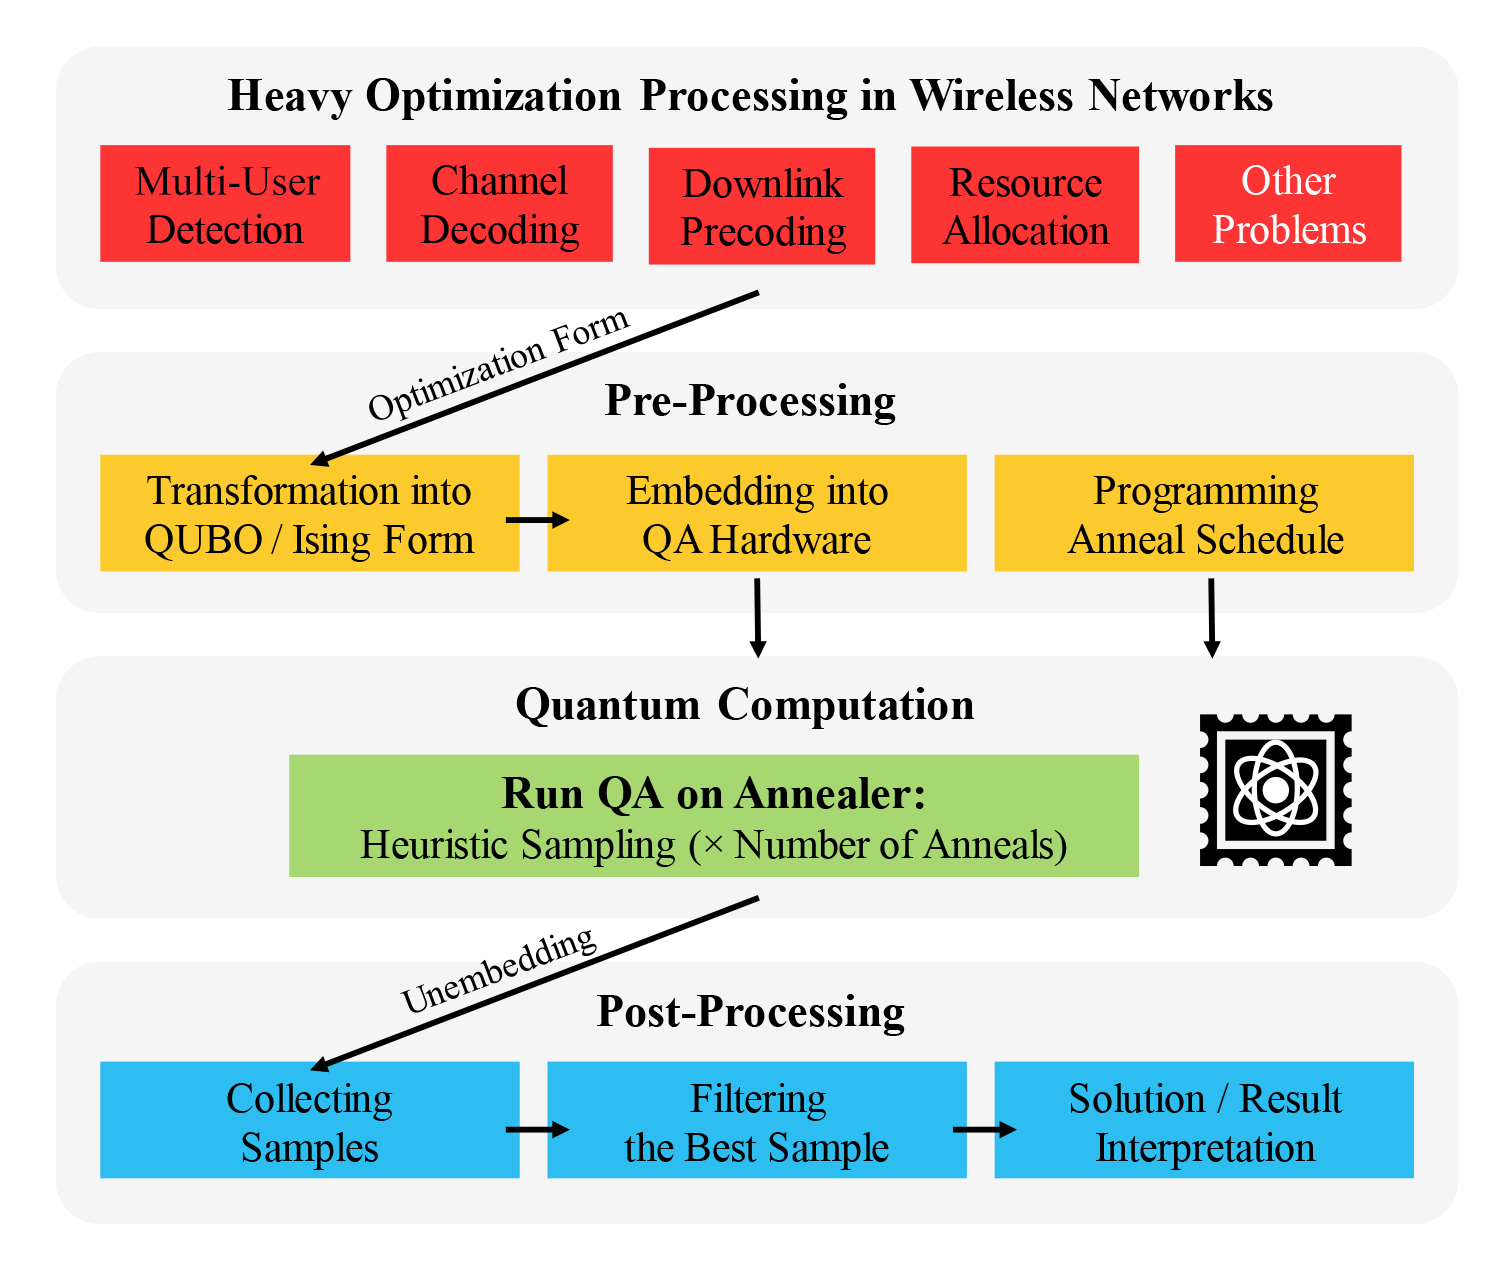
\includegraphics[width=0.8\linewidth]{QAcomms.png}
\caption{The general workflow of QA-based optimization in wireless networks.}
\label{fig:QAcomms}
\end{figure}

This project will particularly focus on the application of QA in multiuser detection for Non-Orthogonal Multiple Access (NOMA), a promising technique that enhances spectral efficiency and supports a higher user density in network environments. The inherent complexity of decoding overlapping signals in NOMA systems presents substantial computational demand. Conventional algorithms often fall short in efficiency, especially as the scale of networks expands.

By adopting QA, we aim to leverage its computational capabilities to explore solutions more efficiently than classical computational approaches allow. The following chapter will delve into the specifics of how quantum annealing is implemented to optimize ML multiuser detection processes in NOMA, highlighting both theoretical advancements and practical applications in current network scenarios.


%%----Experimental Results----%%

\chapter{Leveraging Quantum Annealing for Maximum-Likelihood NOMA Processing in Centralized Radio Access Networks}\label{experimental-results}

This chapter explores the application of QA) to expedite the computations required for NOMA within the framework of C-RAN. We consider a scenario in which a quantum computer, integrated with C-RAN computational resources in a data center, is interconnected with Access Points (APs) via high-speed, low-latency fiber or millimeter-wave links.

Optimization has been identified as one of the key short-term applications where quantum computing may offer significant benefits, even before quantum processors evolve into scalable, error-corrected, and universally capable devices. Although the effectiveness of NISQ devices for optimization tasks remains to be conclusively proven, there is potential for these devices to achieve polynomial or exponential speedups over the best known classical algorithms. Insights from current quantum computing prototypes are crucial for designing practical systems, as real-world performance is difficult to predict or simulate, especially in the presence of device-specific noise.

This chapter outlines the application of QA to the complex task of NOMA decoding within a centralized RAN architecture. Initially, the problem of ML NOMA decoding is reduced to a format processable by a QA solver. The chapter progresses by discussing the practical implementation and performance evaluation of this approach.

\textbf{Chapter Roadmap:} The discussion begins with Section 4.1, which details the \textit{system model for practical NOMA}, setting the stage for subsequent technical developments. Section 4.2 describes the \textit{formulation of the NOMA machine learning problem into a QUBO format}, suitable for QA. Section 4.3 focuses on the \textit{implementation} of this formulation on quantum annealing hardware, and Section 4.4 presents an \textit{evaluation} of the system's performance, analyzing how effectively quantum annealing can optimize NOMA decoding.

By the end of this chapter, the discussions will have demonstrated the potential and practical considerations of applying quantum annealing to improve the efficiency and capability of NOMA systems in real-world telecommunications environments.
\section{System Model}
\label{section:system_model}

We consider a system that exemplifies an uplink NOMA configuration involving a base station (BS) and $N$ end-users, denoted by $U_k$, where \(k \in \mathcal{A} = \{1, 2, \ldots, N\}\). Each node, including the BS and end-users, is equipped with a single antenna. In this NOMA setup, all users simultaneously transmit their data to the BS. The received signal at the BS is a composite of all transmitted signals, modulated by their respective channel gains and added noise, expressed as:

\begin{equation}
y = \sum_{k=1}^{N} s_k h_k + n,
\end{equation}

where $s_k$ is the transmitted symbol of user $k$, with the transmit power defined by an average power constraint $\mathbb{E}\{{s_k s_k^*}\} = P_k$, assumed equal for simplicity, thus $P = P_1 = P_2 = \ldots = P_N$. The wireless channel between each user $U_k$ and the BS is denoted by $h_k$. These channel gains are independent and identically distributed random variables that follow Rayleigh fading, and subject to log-distance path-loss model capturing the stochastic nature of wireless communications:

\begin{equation}
h_k = \frac{\tilde{h}_k}{\sqrt{d_k^\tau}},
\end{equation}

\begin{itemize}
\item $\tilde{h}_k$ represents the Rayleigh fading component, modeled as independent and identically distributed (i.i.d.) random variables (RVs). This component introduces the necessary randomness to account for the multipath effects and other variations in the channel.
\item $d_k$ is the distance of the $k$-th user from the BS, which influences the signal attenuation due to spreading and absorption over the path.
\item $\tau$ is the path-loss exponent, a parameter that depends on the specific environment (e.g., urban, suburban) and dictates how quickly the signal power decreases with distance.
\end{itemize}

\begin{figure}[H]
    \centering
    \includegraphics[width=1\linewidth]{model final111.png}
    \caption{Proposed system model for evaluation.}
    \label{fig:enter-label}
\end{figure}
The term $n$ in Eq.(4.1) denotes the additive white Gaussian noise (AWGN) at the BS with zero mean and variance $\sigma_n^2$.

The power domain NOMA requires that each user's signal arrives at the BS with distinct power levels, typically ensured through varying transmission powers or path losses in the downlink. In our model of uplink NOMA, the distinction in power levels is inherently achieved through the differences in the channel gains $h_k$, assuming users are geographically spaced such that their signals inherently arrive at different power levels at the BS. We consider users geographically distributed such that the closest and farthest users are located 100 m and 500 m from the BS, respectively, with others evenly spaced in between. This setup ensures that signals from different users arrive at the BS with distinct power levels.

The detection at the BS is performed using Maximum Likelihood (ML) detection to decode the received superimposed signal. The goal of ML detection is to estimate the transmitted symbols from all users by minimizing the squared difference between the received signal and the hypothesized signals based on possible transmit symbol vectors. The ML estimation for each user symbol vector ${\hat{s}_1, \hat{s}_2, \ldots, \hat{s}_N}$ that minimizes the residual sum of squares is given by:
\begin{equation}
    \hat{\mathbf{s}}_{ML} = \underset{\hat{s}_1, \hat{s}_2, \ldots, \hat{s}_N}{\arg \min} \left\| y - \mathbf{H}\mathbf{s} \right\|^2,
\end{equation}

where $\mathbf{s} = [s_1, s_2, \ldots, s_N]$ is the vector of transmitted symbols, and $\mathbf{H} = [h_1, h_2, \ldots, h_N]$ is the vector of channel gains. We assume perfect channel estimation at the BS, i.e., the channel gains of each user are known. 

This system model provides a comprehensive framework for analyzing the performance of uplink NOMA networks under realistic channel conditions and user distributions. It  forms the basis for subsequent simulations and performance evaluations discussed in the following sections, focusing on the application of QA to enhance ML decoding processes.

\section{Formulation of the NOMA ML Problem in a QUBO Model}
This section outlines the transformation of the NOMA Maximum Likelihood (ML) detection problem -as previously described in the system model- into a QUBO framework suitable for Quantum Annealing. 
The essence of this transformation lies in encoding the optimization problem such that the solution to the objective function with the lowest energy state corresponds to the optimal solution of the original problem.

The QUBO formulation is typically represented by an upper-diagonal matrix \(Q\), where each element \(q_i\) within the matrix is a binary variable, and the relationship between these variables is governed by:
\begin{equation}
\hat{q}_1, \hat{q}_2, \ldots, \hat{q}_M = \underset{\hat{q}_1, \hat{q}_2, \ldots, \hat{q}_M}{\arg \min} \sum_{i \leq j}^{M} Q_{ij} q_i q_j
\label{qubo}\end{equation}
Here, \(M\) indicates the number of qubits, and the quadratic and linear coefficients are encoded within the matrix \(Q\), with diagonal elements \(Q_{ii}\) and off-diagonal elements \(Q_{ij}\) respectively. Utilizing the property that \(q_i^2 = q_i\).

The ML detection problem, specifically for NOMA, involves finding the symbol vector that minimizes the Euclidean distance between the predicted and actual received signals. To effectively handle the complexities introduced by the superposition of signals in a NOMA system, our approach focuses on the received signal model at the base station (BS). Both the received signal \(y\) and the channel coefficients \(h_k\) are expressed in terms of their real and imaginary components due to broadcast transmission, allowing for a more tractable representation in the quantum domain:
\begin{align}
y &= y_R + jy_I \tag{4.5a} \\
h_k &= h_{k,R} + jh_{k,I} \tag{4.5b}
\end{align}
Each symbol \(s_k\), transmitted by user \(k\), is then transformed into a binary qubit form. The exact representation of these symbols in binary form, and the subsequent construction of the QUBO model, depends on the type of modulation used -described by constellation points as illustrated in \autoref{fig:cons}. 
\begin{figure}
    \centering
    \includegraphics[width=0.75\linewidth]{cons.png}
    \caption{Constellations of different modulation schemes.}
    \label{fig:cons}
\end{figure}

We represent each of the $k$ senders' candidate symbols $s_k \in O$ (where $1 \leq i \leq k$), 
with $\log_2(|O|)$ QUBO solution variables, naturally requiring $M = k \cdot \log_2(|O|)$ QUBO 
variables for $k$ transmitters, and form these QUBO variables into a vector $q_i$ for each 
sender $k$: $q_i = [q_{(i-1) \cdot \log_2(|O|) + 1}, \ldots, q_{i \cdot \log_2(|O|)}$]
,This directly affects the complexity and structure of the QUBO matrix \cite{Kim2019}.


The subsequent sections will detail specific transformations for different modulation schemes such as BPSK, QPSK, 16-QAM, and 64-QAM, and explore how each scheme’s characteristics influence the QUBO formulation and strategies for efficient quantum annealing.

\subsubsection*{BPSK Modulation}
In the BPSK modulation scheme, each symbol \(s_k\) can take values from the set \(\{+1, -1\}\). These symbols can be reformulated into the QUBO form by using the binary transformation \(s_k = 2q_k - 1\), where \(q_k \in \{0,1\}\) represents the binary state of user \(k\)'s symbol. Here, \(M\) in the QUBO equation corresponds to \(N\), the number of users.

To derive the QUBO coefficients, we start by considering the objective function that arises from the ML detection of the received signals\cite{Kizilirmak2020}, expanding the norm:
\vspace{-0.1cm}
\begin{align}
||y - \mathbf{s H}||^2 &= \left| \left|y - \sum_{k=1}^{N} s_k h_k\right| \right|^2 \nonumber \\
&= \left| \left| y - \sum_{k=1}^{N} (2q_k - 1) h_k\right| \right|^2 \nonumber \\
&= \left| \left| \left(y + \sum_{k=1}^{N} h_k\right) - 2 \sum_{k=1}^{N} h_k q_k\right| \right| ^2 \nonumber \\
&= \left(y + \sum_{k=1}^{N} h_k\right)^2 + 4 \sum_{k=1}^{N} h_k^2 q_k^2 - 4\left(y + \sum_{k=1}^{N} h_k\right) \sum_{k=1}^{N} h_k q_k + 8 \sum_{i=1}^{N} \sum_{j=i+1}^{N} h_i h_j q_i q_j.
\end{align}

Simplifying and rearranging by breaking down the received signal \(y\) and the channel coefficients \(h_k\) into their real and imaginary parts, where \(y = y_{\rm R} + jy_{\rm I}\) and \(h_k = h_{k,{\rm R}} + jh_{k,{\rm I}}\):
\vspace{-0.05cm}
\begin{align}
||y - \mathbf{s H}||^2 &= \left(y_{\rm R} + \sum_{k=1}^{N} h_{k,{\rm R}}\right)^2 + \left(y_{\rm I} + \sum_{k=1}^{N} h_{k,{\rm I}}\right)^2 \nonumber \\
&\quad + 4 \sum_{k=1}^{N} \left(h_{k,{\rm R}}^2 + h_{k,{\rm I}}^2\right) q_k \nonumber \\
&\quad - 4\left(y_{\rm R} + \sum_{k=1}^{N} h_{k,{\rm R}}\right) \sum_{k=1}^{N} h_{k,{\rm R}} q_k - 4\left(y_{\rm I} + \sum_{k=1}^{N} h_{k,{\rm I}}\right) \sum_{k=1}^{N} h_{k,{\rm I}} q_k \nonumber \\
&\quad + 8 \sum_{i=1}^{N} \sum_{j=i+1}^{N} \left(h_{i,{\rm R}} h_{j,{\rm R}} + h_{i,{\rm I}} h_{j,{\rm I}}\right) q_i q_j.
\end{align}

Grouping and identifying the linear terms (multiplied by only one binary variable \( q_k \)) and quadratic terms (involving two binary variables \( q_i \) and \( q_j \)), leads us to the QUBO coefficients \cite{Gabdulsattarov2023}:\footnote{Note that the equations involving the positive integer variables \(i\) and \(j\) must satisfy the condition \(i < j\).}
\begin{align}
Q_{ii}^{\rm B} &= P \left[ -4 h_{i,{\rm R}} \left( \sum_{l=1}^{N} h_{l,{\rm R}} - h_{i,{\rm R}} \right) - 4 h_{i,{\rm I}} \left( \sum_{l=1}^{N} h_{l,{\rm I}} - h_{i,{\rm I}} \right) \right] \nonumber \\
&\quad - \sqrt{P} \left( 4 y_{\rm R} h_{i,{\rm R}} + 4 y_{\rm I} h_{i,{\rm I}} \right), \\
Q_{ij}^{\rm B} &= P \left( 8 h_{i,{\rm R}} h_{j,{\rm R}} + 8 h_{i,{\rm I}} h_{j,{\rm I}} \right).
\end{align}
\subsubsection{QPSK Modulation}
Quadrature Phase Shift Keying (QPSK) modulation uses four points on the constellation diagram, equally spaced around a circle. Each symbol in QPSK, \(s_k\), is represented by a complex number of the form \(\{\frac{\pm1 \pm j}{\sqrt{2}}\}\), as illustrated in \autoref{fig:cons} residing on a unit circle with \(90^\circ\) phase differences between consecutive symbols. This phase difference allows each symbol to be represented by two qubits. Therefore, for the formulation in the QUBO model, \(M\) becomes \(2N\), where \(N\) is the number of users, effectively doubling the number of binary variables required.

The representation of QPSK symbols in QUBO is given by:
\begin{equation}
    s_k = \left[\left(2q_{2k-1}-1\right) + j\left(2q_{2k}-1\right)\right]/\sqrt{2}
\end{equation}



The corresponding QUBO matrix coefficients for the QPSK modulation are derived from the real and imaginary parts of the received signals and the channel coefficients, following the method previously discussed for BPSK \cite{Gabdulsattarov2023}:

\begin{figure}[H]
	\begin{align}
		Q_{(2i-1),(2i-1)}^{\rm Q} &= \frac{P}{2} \left[ -4 h_{i,{\rm R}} \left(
		\left( \sum_{l=1}^{N} h_{l,{\rm R}} - h_{i,{\rm R}} \right) - \left( \sum_{l=1}^{N} h_{l,{\rm I}} - h_{i,{\rm I}} \right)
		\right) \right. \nonumber \\
		&\quad \left. - 4 h_{i,{\rm I}} 
		\left(
		\left( \sum_{l=1}^{N} h_{l,{\rm R}} - h_{i,{\rm R}} \right) + 
		\left( \sum_{l=1}^{N} h_{l,{\rm I}} - h_{i,{\rm I}} \right)
		\right)
		\right] \nonumber \\
		&\quad - \sqrt{2 P} \left( 2 y_{\rm R} h_{i,{\rm R}} 
		+ 2 y_{\rm I} h_{i,{\rm I}} \right), \label{eq:Q1} \\
		Q_{(2i),(2i)}^{\rm Q} &= \frac{P}{2} \left[ -4 h_{i,{\rm R}} \left(
		\left( \sum_{l=1}^{N} h_{l,{\rm R}} - h_{i,{\rm R}} \right) + \left( \sum_{l=1}^{N} h_{l,{\rm I}} - h_{i,{\rm I}} \right)
		\right) \right. \nonumber \\
		&\quad \left. - 4 h_{i,{\rm I}} 
		\left(
		-\left( \sum_{l=1}^{N} h_{l,{\rm R}} - h_{i,{\rm R}} \right) + 
		\left( \sum_{l=1}^{N} h_{l,{\rm I}} - h_{i,{\rm I}} \right)
		\right)
		\right] \nonumber \\
		&\quad - \sqrt{2P} \left( -2 y_{\rm R} h_{i,{\rm I}} 
		+ 2 y_{\rm I} h_{i,{\rm R}} \right). \label{eq:Q2}
	\end{align}
\end{figure}
\vspace{-1cm}
\begin{equation}
    Q_{(2i-1),(2i)}^{\rm Q} = 0, \quad \forall i \ge 1, 
\end{equation}
\vspace{-1cm}
\begin{align}
    Q_{(2i-1),(2j-1)}^{\rm Q} &= Q_{(2i),(2j)}^{\rm Q} = \frac{P}{2} \left( 8 h_{i,{\rm R}} h_{j,{\rm R}} + 8 h_{i,{\rm I}} h_{j,{\rm I}} \right), \\
    Q_{(2i-1),(2j)}^{\rm Q} &= \frac{P}{2} \left( 8 h_{i,{\rm I}} h_{j,{\rm R}} 
    - 8 h_{i,{\rm R}} h_{j,{\rm I}} \right), \\
    Q_{(2i),(2j-1)}^{\rm Q} &= \frac{P}{2} \left( -8 h_{i,{\rm I}} h_{j,{\rm R}} 
    + 8 h_{i,{\rm R}} h_{j,{\rm I}} \right).
\end{align}

\subsubsection{16-QAM Modulation}
The 16-QAM modulation scheme encodes four information bits into one complex symbol, resulting in a constellation with 16 distinct points. These symbols are represented as $ s_{k} \in \{\pm b\pm jb, \pm b\pm j3b, \pm 3b\pm jb, \pm 3b \pm j3b\} $, where $b = 1/(3\sqrt{2})$. To incorporate these symbols into the QUBO model, each symbol $s_k$ is encoded using four qubits:

\begin{equation}
    s_{k} = \left[\left(4q_{4k-3}+2q_{4k-2}-3\right) + j\left(4q_{4k-1}+2q_{4k}-3\right)\right]/3\sqrt{2}.
\end{equation}

\vspace{-0.3cm}
Here, $M$ in \eqref{qubo} is extended to four times the number of users, i.e., $4N$. The coefficients for the QUBO model will be detailed in \autoref{Chapter:append}1, following the method previously discussed.

\subsubsection{64-QAM Modulation}
64-QAM, an even more densely packed modulation scheme, encodes six bits per symbol, creating a constellation with 64 points. The symbols are defined as:
\[
s_{k} \in \left\lbrace 
\begin{array}{cccc}
	\pm a\pm ja & \pm a\pm j3a & \pm a\pm j5a & \pm a\pm j7a \\
	\pm 3a\pm ja & \pm 3a \pm j3a & \pm 3a\pm j5a & \pm 3a \pm j7a\\
	\pm 5a\pm ja & \pm 5a \pm j3a & \pm 5a\pm j5a & \pm 5a \pm j7a \\
	\pm 7a\pm ja & \pm 7a \pm j3a & \pm 7a\pm j5a & \pm 7a \pm j7a
	\end{array} \right\rbrace,
\]
where $a = 1/(7\sqrt{2})$. Each symbol requires six qubits for representation in the QUBO model:
\begin{equation}
s_{k} = a \left(8q_{6k-5}+4q_{6k-4}+2q_{6k-3}-7\right) + j a \left(8q_{6k-2}+4q_{6k-1}+2q_{6k}-7\right).
\end{equation}

The variable $M$ in \eqref{qubo} increases to six times the number of users, i.e., $6N$. The detailed QUBO coefficients are included in \autoref{Chapter:append}2.

\begin{table}[h]
\centering
\caption{Qubit requirements for different NOMA encoded configurations}
\label{table:noma_qubit_requirements}
\begin{tabular}{@{}ccccc@{}}
\toprule
\multirow{2}{*}{Number of Users} & \multicolumn{4}{c}{Modulation Type} \\ \cmidrule(l){2-5} 
 & BPSK & QPSK & 16-QAM & 64-QAM \\ \midrule
10 & \cellcolor{green!25}10 & \cellcolor{green!25}20 & \cellcolor{green!25}40 & \cellcolor{yellow!40}60 \\
20 & \cellcolor{green!25}20 & \cellcolor{green!25}40 & \cellcolor{green!25}80 & \cellcolor{yellow!40}120 \\
30 & \cellcolor{green!25}30 & \cellcolor{green!25}60 & \cellcolor{yellow!40}120 & \cellcolor{yellow!40}180 \\
40 & \cellcolor{green!25}40 & \cellcolor{green!25}80 & \cellcolor{yellow!40}160 & \cellcolor{yellow!40}240 \\
80 & \cellcolor{green!25}80 & \cellcolor{yellow!40}160 & \cellcolor{yellow!40}320 & \cellcolor{red!25}480 \\
100 & \cellcolor{green!25}100 & \cellcolor{yellow!40}200 & \cellcolor{yellow!40}400 & \cellcolor{red!25}600 \\
120 & \cellcolor{yellow!40}120 & \cellcolor{yellow!40}240 & \cellcolor{red!25}480 & \cellcolor{red!25}720 \\
140 & \cellcolor{yellow!40}140 & \cellcolor{yellow!40}280 & \cellcolor{red!25}560 & \cellcolor{red!25}840 \\
160 & \cellcolor{yellow!40}160 & \cellcolor{yellow!40}320 & \cellcolor{red!25}640 & \cellcolor{red!25}960 \\
180 & \cellcolor{yellow!40}180 & \cellcolor{yellow!40}360 & \cellcolor{red!25}720 & \cellcolor{red!25}1080 \\
\bottomrule
\end{tabular}
\end{table}
Given a number $M$ of binary variables (i.e., logical qubits) in QUBO form $q_i$, the 
embedding process represents each with a chain of $\lceil M/4 \rceil + 1$ qubits, and requires 
a total of $M \cdot (\lceil M/4 \rceil + 1)$ qubits. Recall that $M = k \cdot \log_2(|O|)$.

\autoref{table:noma_qubit_requirements} summarizes the size of the embedding in logical qubits, as a function of the 
problem's parameters—number of users with single antenna, and modulation type. Color 
coding indicates feasibility, whether or not the given parameters fit into the number 
of qubits available on current D-Wave machines.

\section{Implementation}

The implementation of the quantum annealing (QA) method for signal decoding in a power-domain uplink Non-Orthogonal Multiple Access (UL-NOMA) system was executed using D-Wave’s Advantage QPU. The experiments took advantage of the QPU's parallelization capabilities to optimize efficiency and reduce simulation time significantly. The annealer was programmed to execute multiple annealing cycles with consistent parameters across each cycle to collect robust statistical data. The configuration with the lowest energy from these cycles was selected as the most likely solution.

To manage computation efficiently, the QA setup included running multiple instances simultaneously on the QPU. This parallelization substantially reduced computation time by a factor approximately given by \(P_f \approx \frac{N_{\text{tot}}}{N (\lceil N/4 \rceil + 1)}\), where \(N_{\text{tot}}\) is the total number of instances and \(N\) is the number of qubits involved\cite{Kim2019}. For example, a 16-qubit problem, which represents a 16-user BPSK or an 8-user QPSK, could potentially be executed over 20 times in parallel on the Advantage system.

The waveform generation and signal processing were implemented in Python, except for the parts directly executed by the QA. Conventional decoding techniques such as Successive Interference Cancellation (SIC) and a brute-force solution of Maximum Likelihood (ML) decoding were performed using MATLAB on a machine equipped with an AMD\texttrademark Ryzen 7 processor, 16GB RAM, and an RTX 3060 GPU. These traditional methods provided a basis for comparing the effectiveness and efficiency of quantum annealing against established algorithms.

The annealing time, \(T_{\text{anneal}}\), was set to 20$\mu$s, and the total number of samples, \(N_{\text{total}}\), was fixed at 1000 for each run. Most runs utilized Native Clique Embedding due to its ability to produce uniform chains, leading to more stable outcomes compared to heuristic embedding methods. Table 4.2 lists the used settings. D-Wave 


The decoding time was also recorded to determine the real-time computing demands for NOMA using QA and to compare these demands with other decoding methods. The results and comparisons are discussed in detail in the following evaluation section.
\begin{table}
\caption{D-Wave system parameters.}
\centering
\label{table:dwave_parameters}
\begin{tabular}{l c}
\hline
\textbf{Parameter} & \textbf{Value} \\
\hline
Annealing Time (\(T_{\text{anneal}}\)) & 20 $\mu$s \\
Total Number of Samples (\(N_{\text{total}}\)) & 1000 \\
Version & D-Wave Advantage 5.2 \\
Embedding Type & Native Clique Embedding \\
Chain Strength & 0.3-0.8 \\
\hline
\end{tabular}
\end{table}
\section{Evaluation}

The evaluation of our quantum annealing (QA) implementation for Maximum Likelihood (ML) detection in Non-Orthogonal Multiple Access (NOMA) primarily utilized the Bit Error Rate (BER) as the main performance metric. BER is defined as the ratio of incorrectly decoded bits and is given by:
\begin{equation}
\text{BER}(\hat{b}) = \frac{\|b-\hat{b}\|}{n},
\end{equation}
where \( n \) is the length of the transmitted bit string \( b \), and \( \|b-\hat{b}\| \) represents the number of bits that differ between the transmitted bit string \( b \) and the decoded bit string \( \hat{b} \). This metric was pivotal in assessing the QA's effectiveness in managing the complexities inherent in multi-user detection for PD-NOMA systems. An increase in problem complexity, indicated by higher numbers of users or larger constellations, was expected to yield higher BERs.

A substantial number of simulation runs, in the order of thousands, were executed to ensure statistical significance of the results. The experiments spanned a variety of symmetric user setups typical in commercial telecommunications to confirm the practical relevance of the findings. The quantum annealer was programmed to execute multiple annealing cycles with uniform parameters to compile a robust dataset, where the configuration with the lowest energy among these cycles was considered the optimal solution, the process is outlined in Algorithm \autoref{algorithm}.

BER evaluations were conducted against two main variables: (a) the number of users and, (b) the transmit power for different user distances. This methodical approach allowed thorough examination of the QA's scalability and performance under varying configurations. Additionally, the performance of the QA-based ML detection was benchmarked against conventional decoding techniques, primarily Successive Interference Cancellation (SIC) and brute-force ML decoding performed on MATLAB.

Furthermore, decoding times were meticulously recorded to evaluate the real-time computational demands of NOMA using quantum annealing, highlighting its practical applicability in live telecommunications environments. Results from these comprehensive tests demonstrated that the advanced QPU architectures not only accommodate larger problem sizes but also enhance performance for smaller configurations, validating our hypothesis and underscoring the potential of quantum computing to elevate NOMA systems.

\begin{algorithm}
\caption{Simulation of NOMA on Quantum Annealer \label{algorithm}  }
\begin{algorithmic}[1]
\State \textbf{Input:} Number of users $N$, Modulation type, Transmit power $P$
\State \textbf{Output:} Bit Error Rate (BER)

\Procedure{Simulate NOMA}{$N$, Modulation, $P$}
    \State Generate bits according to $N$ and Modulation type
    \State Generate channel gains $h$ with i.i.d. Rayleigh fading
    \State Calculate path loss based on users' distances
    \State Generate AWGN $n$ with specified variance
    \State Compute received signal $y$ at BS using $h$, path loss, $P$, and $n$
    \State Calculate QUBO coefficients using $h$, $y$, and $P$
    \If{Number of users and modulation type are unchanged}
        \State Use existing embedding
    \Else
        \State Generate embedding using MinorMiner
    \EndIf
    \State Send coefficients and embedding to D-Wave for annealing
    \State Obtain SampleSet from D-Wave QPU
    \State Select first sample from SampleSet (lowest energy)
    \State Transform QUBO variables back to bits or symbols
    \State Compare the decoded bits/symbols against the original
    \State Calculate error and accumulate over many iterations
    \State Compute BER
    \State \textbf{return} BER
\EndProcedure
\end{algorithmic}
\end{algorithm}




\subsection{Understanding Empirical Results}

When running a problem on a quantum annealer, the machine returns a sample set containing solutions ranked by their energy levels, with the lowest energy solution being the most optimal. The number of reads performed during the quantum annealing process determines the size of the sample set. Each solution in the sample set may occur multiple times, as the same solution can be found in different reads.

Among these, multiple occurrences of a certain spin configuration (with agreeing spin variables) are very likely to be observed, which could be used to identify spins easy (or hard) to detect (i.e., variables that are very likely to be assigned a certain value in the unknown optimal ML solution). \autoref{fig:empirical} shows an illustrative example of detecting a received \(1 \times 1\) QPSK signal \(y\) in two equivalent representations, one in the I-Q plane with Euclidean distance $\mathcal{D}$ (left), and the other with Ising energies $\mathcal{H}(s)$ (right). In this example, the first spin variable \(s_1\) (corresponding to the symbol’s real part) is likely to be detected as +1 for most PMIS runs, since the difference in Ising energy from all configurations that have \(s_1 = +1\) (resulting in $\mathcal{H}_3$ or $\mathcal{H}_4$ in Figure 4.5, right) and \(s_1 = -1\) (resulting in $\mathcal{H}_1$ or $\mathcal{H}_2$ in \autoref{fig:empirical}, right) is significant. The spin \(s_1\) is easy to detect compared to spin \(s_2\) (corresponding to the symbol’s imaginary part). Multiple occurrences of QA runs agreeing on \(s_1 = +1\) indicate this, while QA runs will disagree on the value of \(s_2\), because the two most frequent spin configurations’ energies ($\mathcal{H}_3$ and $\mathcal{H}_4$) themselves disagree on the value of \(s_2\).
\begin{figure}
    \centering
    \includegraphics[width=1\linewidth]{empirical.png}
    \caption{Equivalent representations of $1 \times 1$ QPSK detection: Euclidean distances $\mathcal{D}(v)$ in the I-Q plane (left), and Ising energies $\mathcal{H}(s)$ (right). Shadings highlight likely solutions.}
    \label{fig:empirical}
\end{figure}
This phenomenon is even more pronounced in higher-order modulations like 16-QAM, where each symbol is represented by multiple spins. In such cases, the mapping complexity increases as each spin or group of spins corresponds to different segments of the encoded symbol. For instance, odd and even-numbered spins might determine different quadrants and positions within these quadrants in the symbol constellation. This differentiation helps in identifying which spins are more susceptible to noise and which are more robust, thereby aiding in more accurate symbol reconstruction.

The D-Wave inspection tool provides valuable insights into the quantum annealing results. It allows users to view the histogram of the sample set, which displays the distribution of solutions and their corresponding energy levels. This histogram helps in understanding the frequency of occurrence for each solution and the relative energy differences between them. Furthermore, the inspection tool visualizes how the problem is embedded in the quantum processing unit (QPU) as visulized in \autoref{fig:inspect}. As explained earlier, the logical qubits of the problem are mapped onto the physical qubits of the QPU, taking into account the connectivity constraints of the hardware. The inspection tool provides a graphical representation of this embedding, enabling users to see how the problem is physically represented on the QPU.
\begin{figure}[H]
    \centering
    \includegraphics[width=1\linewidth]{dwaveinspect.png}
    \caption[Dwave problem inspector.]{Dwave problem inspector displaying the embedded problem(left), and the returned energies histogram(right), for the case of 10-user BPSK.}
    \label{fig:inspect}
\end{figure}
In addition to the histogram and embedding visualization, the inspection tool also provides execution timing information. This includes details such as the total execution time, the time spent on problem initialization, the actual annealing time, and the time taken for readout. These timing metrics can be useful for analyzing the performance of the quantum annealing process and identifying potential bottlenecks.

\subsection{Bit-Error Rate Performance for QA Based Maximum-Likelihood  Versus. Number of Users Across Various Modulation Schemes}
%In our study, we examine the impact of user density per cell on the Bit Error Rate (BER) across various modulation schemes within a Non-Orthogonal Multiple Access (NOMA) system. The testing environment was standardized with the transmit power set to 10 dBm and the Ambient White Gaussian Noise (AWGN) power fixed at -60 dBm.

%Initially, at lower user densities, all modulation schemes maintain a relatively low BER, demonstrating the effectiveness of Quantum Annealing (QA) in simpler communication scenarios. This indicates robust initial decoding capabilities when the system is not heavily loaded. However, as the number of users increases, there is a noticeable degradation in BER performance across all modulation schemes. This degradation reflects the increasing challenges QA faces in accurately decoding superposed signals from multiple users.

%Among the modulation schemes analyzed, BPSK exhibits the best resilience, with a slower increase in BER as user numbers increase. It manages to maintain an average BER below $10^{-3}$ until the user count exceeds 16, suggesting that it can support a higher number of users without significant performance degradation. QPSK shows comparable performance to BPSK for user counts lower than 6 but begins to falter beyond this point. Conversely, higher-order modulations like 16QAM and 64QAM display a rapid increase in BER even with few users, managing a BER better than $10^{-2}$ only for groups smaller than 3 users. These higher-order modulations are significantly impacted by their denser signal constellations, which are more susceptible to noise and interference.

%As user density grows, the challenge for QA in differentiating closely spaced signal states intensifies, especially for higher-order modulations where denser constellation diagrams lead to a higher likelihood of phase or amplitude errors during decoding processes. Our findings indicate distinct capacity limits for each modulation type based on where the BER begins to sharply increase. For instance, while BPSK can support more than 16 users before reaching unacceptable BER levels, 16QAM and 64QAM struggle beyond 3 users. 

%This analysis not only aids in understanding the performance limits of different modulation schemes under QA but also assists in planning and optimizing network configurations for varied user densities and communication demands in NOMA systems.



In \autoref{fig:num}, The impact of user density per cell on the Bit Error Rate (BER) when using Quantum Annealing (QA) for maximum likelihood decoding across various modulation schemes is evaluated within a Non-Orthogonal Multiple Access (NOMA) system. The test conditions were standardized with the transmit power set at 10 dBm and the Additive White Gaussian Noise (AWGN) power fixed at -40 dBm.
\begin{figure}[h]
    \centering
    \includegraphics[width=0.85\linewidth]{Chapter3/Figs/num.png}
    \caption{BER vs. the number of users per cell under various modulation schemes.}
    \label{fig:num}
\end{figure}
As expected, the average BER performance degrades with the increase in the number of users per cell. Initially, at lower user densities, The proposed QA ML decoder demonstrates a capability to maintain relatively low BER values, suggesting effective decoding when the system is under lighter loads. However, as the number of users per cell increases, there is a noticeable increase in BER across all modulation schemes, indicating the growing complexity that QA needs to manage for decoding superposed signals from multiple users.

BPSK, being the simplest modulation, shows the least increase in BER as the number of users grows, maintaining an average BER of $10^{-3}$ until the user count exceeds 16. This points to a more efficient decoding by the proposed QA Maximum-Likelihood under BPSK modulation at higher user densities compared to more complex modulations. QPSK, while performing comparably to BPSK for fewer than 6 users, also begins to show performance decline as the number of users increase. Conversely, complex schemes like 16QAM and 64QAM achieving an average BER  exhibit rapid increases in BER with just a small addition of users, highlighting their sensitivity to decoding errors under QA due to their denser signal constellations.

%The increase in user density denotes the challenge for the proposed detector in differentiating closely spaced signal states, which is especially marked in higher-order modulation schemes. These findings underscore distinct limits on the capacity of QA for decoding each modulation type as the BER sharply rises at higher user densities.For instance, while BPSK and QPSK allows for more users before the BER becomes unacceptable, 16QAM and 64QAM did not perform adequately beyond 3 users.
The performance of the QA ML decoder is highlighted by its ability to maintain relatively low BER for a reasonable number of users in simpler modulation schemes. However, for higher-order modulation schemes, the BER increases rapidly, suggesting a limitation in handling more complex modulation with an increasing number of users.
By setting a threshold BER for outage probability at say $10^{-2}$ , we can strategically determine an optimal number of users for each modulation type for further detailed analysis. For instance, BPSK can support up to 16 users, and QPSK can support up to 6 users while maintaining the acceptable BER. Higher-order modulation schemes like 16QAM and 64QAM can not achieve acceptable BER for more than 3 users.
\vspace{1cm}
\begin{table}[ht]
\centering
\caption{Simulation parameter settings.}
\label{tab:simulation_parameters}
\begin{tabular}{>{\bfseries}l l}
\toprule
Parameter                           & Value \\
\midrule
Modulation Schemes                  & BPSK, QPSK, 16-QAM, 64-QAM \\
Distance from User to Base Station  & 100 $-$ 500 m \\
Channel Fading                      & Rayleigh \\
Pathloss Model                      & Log-distance \\
Environment                      & Urban cellular radio \\
Pathloss exponent                      & 2.7 \\
Transmit Power                      & -30 $-$ 30 dBm \\
AWGN Noise Power                    & -30 dBm \\
Number of Users per Cell            & 2 $-$ 20 \\
\bottomrule
\end{tabular}
\end{table}

\subsection{Bit-Error Rate Performance for QA Based Maximum-Likelihood detection with BPSK modulation}
After analyzing the previous plot for BER versus the number of users, A 10 user scenario was selected for detailed analysis based on the performance degradation observed beyond this point, particularly under BPSK modulation. The decoding effectiveness of Maximum Likelihood (ML) brute force solution BF, ML Quantum Annealing (QA), and Successive Interference Cancellation (SIC) in terms of BER performance across varying transmit powers were compared against each-other. with the noise power set to -30dbm QA was simulated for particular transmit power levels, i.e., \( P = \{-30, -20, -10, 0, 10, 20, 30\} \) dBm, other simulation parameters showcased in \autoref{tab:simulation_parameters}
\begin{figure}[h]
    \centering
    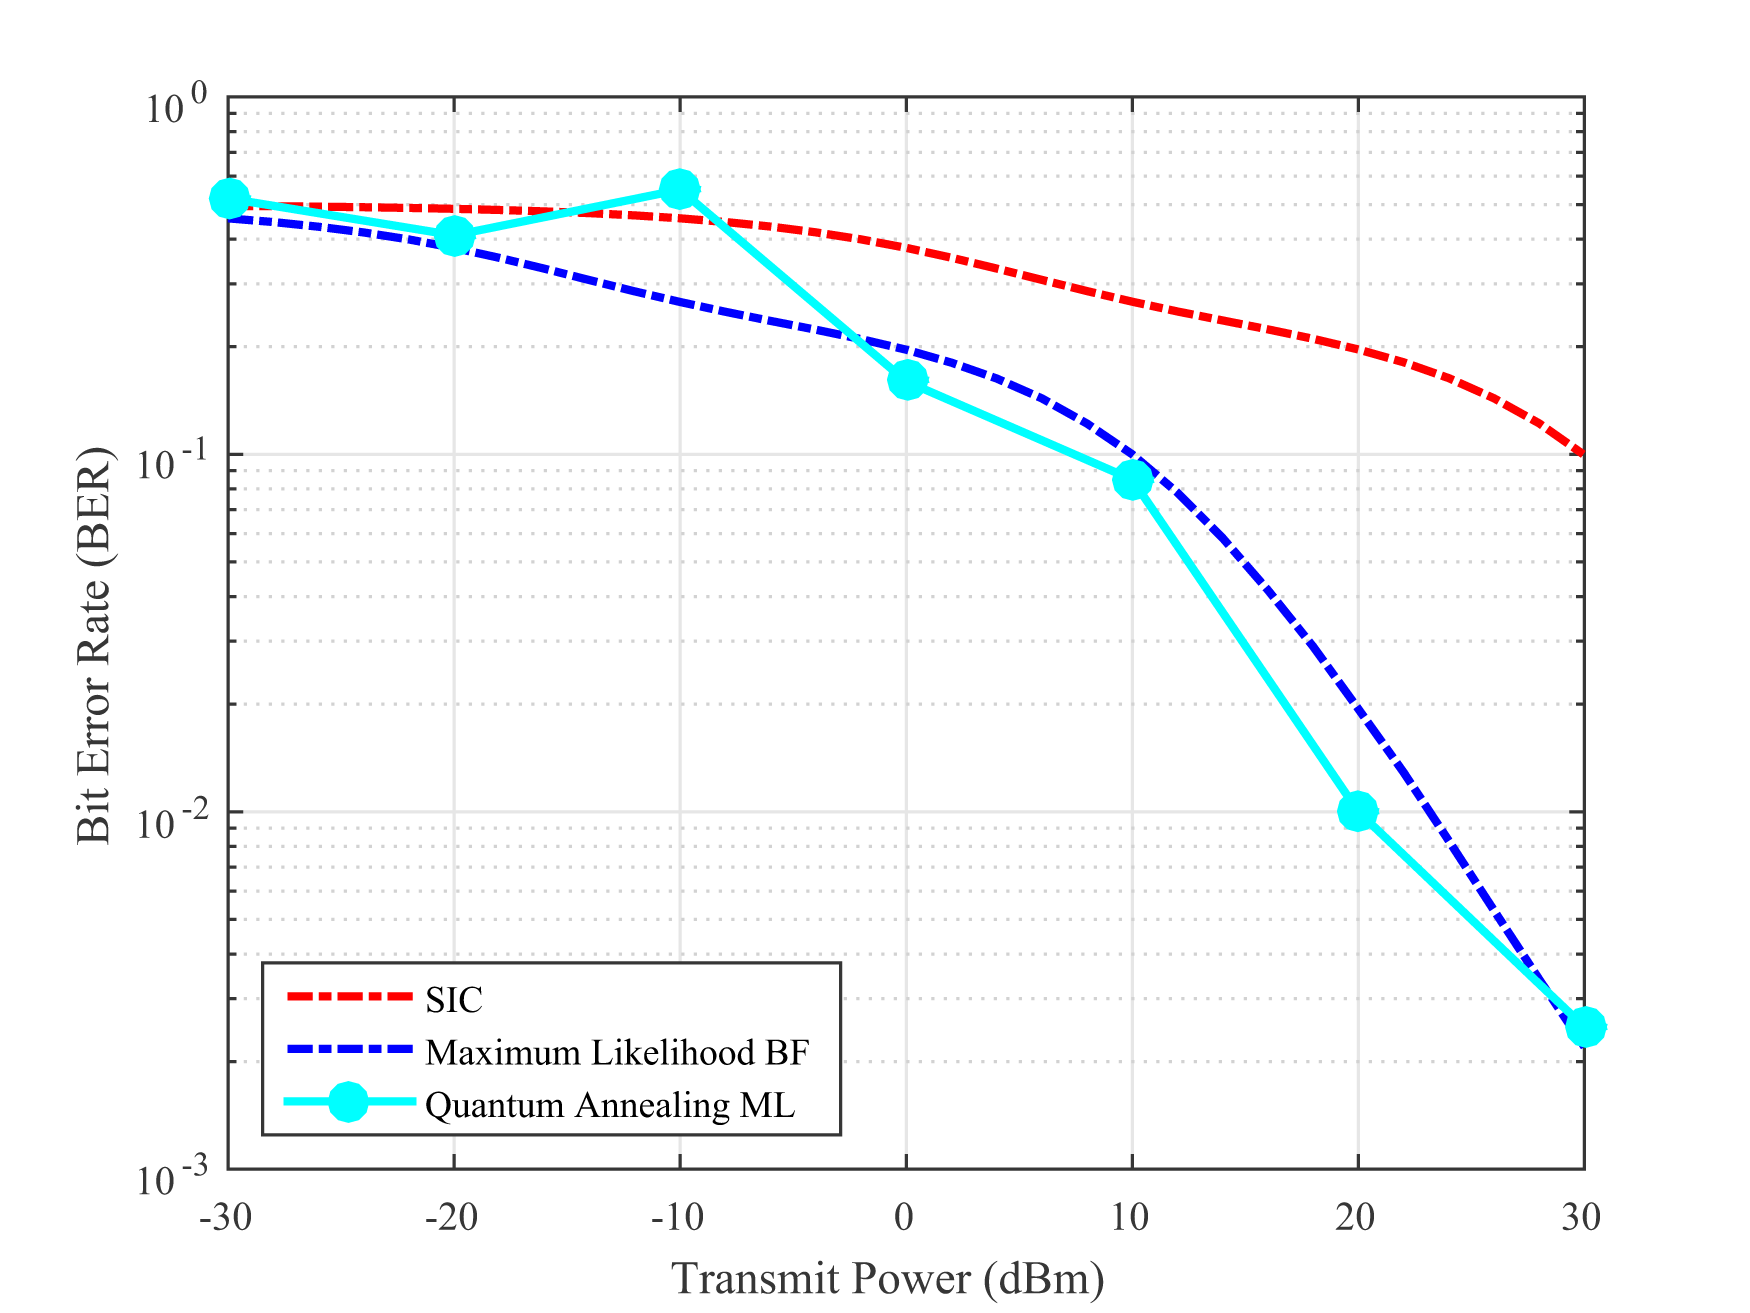
\includegraphics[width=0.85\linewidth]{Chapter3/Figs/bpskvs copy.png}
    \caption{The avergae BER performance vs. the transmit power for a 10 user NOMA scenario employing BPSK, with different decoding techniques.}
    \label{fig:bpskvs}
\end{figure}

\autoref{fig:bpskvs} illustrates the BER performances of each decoding
method. The BER curves can be characterized by different behaviour. The findings show that the 3 methods performances coincide up to -20 dBm, and then the bruteforce ML starts outperforming both SIC and QA over a short transmit power range (i.e, 15 dbm to -5 dbm). However, afterwards, SIC starts
experiencing noticeable performance degradation while ML brute force consistently reduces BER with increased power, demonstrating robust decoding, ML QA improves significantly at higher power levels, providing identical or even lower BER than BF. 
In general, the QA, BF and SIC curves follow the same trend till 10 dBm, but after this level,
the SIC performance degrades substantially, while the BER
result of QA is approximately the same as BF. The reason
for the SIC’s low performance could be insufficient differences
between the end-users’ power levels.
%SIC's performance varied depending on interference and power levels.
\begin{figure}[H]
    \centering
    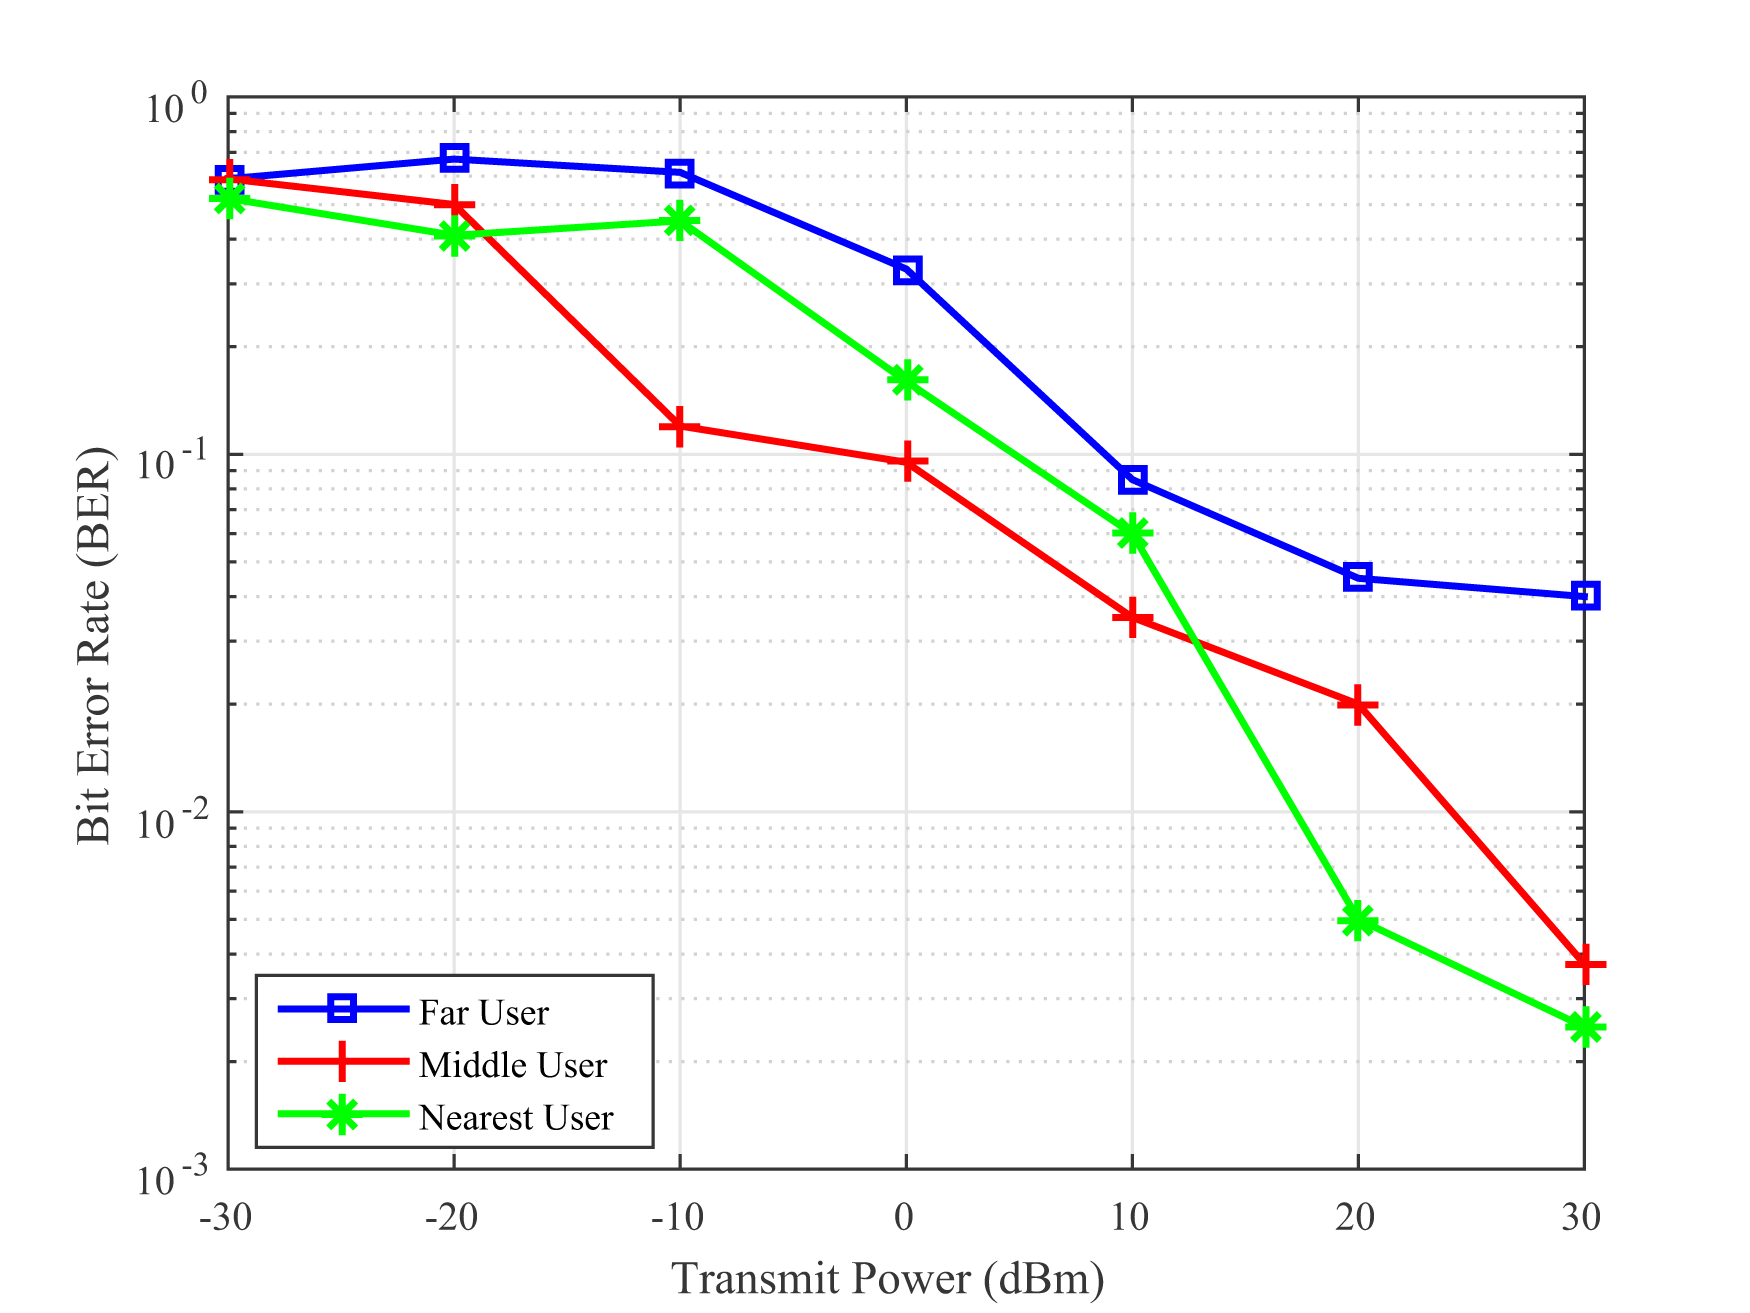
\includegraphics[width=0.85\linewidth]{Chapter3/Figs/bpsk10 copy.png}
    \caption{The BER performance vs. the transmit power per user at different cell positions—near, middle, and far- for BPSK with Quantum Annealing based maximum likelihood decoder.}
    \label{fig:bpsk10}
\end{figure}

\autoref{fig:bpsk10} shows in-depth analysis of ML QA performance employing BPSK modulation for each user at different cell positions—near, middle, and far— the plot revealed that the 3 users have similar performance upto -25 dbm, the middle user performance enhances considerably, while the far and near user follow the same trend.  
A sharp decrease in BER is noticed the near user performance after 10 dbm power, while the Far user demonstrates a slowly improving trend and the middle user exhibits a steady improvement in BER as the transmit power increases.
Overall, while both near and far users experience better performance in terms of BER, the difference in improvement between them is small.

\subsection{Bit-Error Rate Performance for QA Based Maximum-Likelihood detection with QPSK modulation}
For QPSK, a simulation identical to that conducted for BPSK was performed for 5-user cell. In \autoref{fig:qpskvs}, the comparison reveals that SIC, BF, and QA perform similarly up to approximately -10 dBm. After this threshold, BF begins to outperform the other methods. QA and SIC maintain similar BER levels until 0 dBm, after which QA experiences a substantial improvement, reaching parity with BF at 10 dBm. Meanwhile, SIC starts to experience noticeable performance degradation.


\begin{figure}[H]
    \centering
    \includegraphics[width=0.85\linewidth]{Chapter3/Figs/qpskvs copy.png}
    \caption{The avergae BER performance vs. the transmit power for a 5 user NOMA scenario employing QPSK, with different decoding techniques.}
    \label{fig:qpskvs}
\end{figure}

the performance of the ML QA decoder employing QPSK modulation for users located at different positions within a cell is depicted in \autoref{fig:qpsk5}. Initially, all users types exhibit comparable BER performance up to approximately -20 dBm of transmit power. As the transmit power increases beyond this point, the performance begins to diverge.

For the far user, the BER gradually improves with increasing transmit power, indicating a slow but steady enhancement in performance. The BER remains relatively high until about 10 dBm, where a more pronounced improvement is observed.
\begin{figure}[H]
    \centering
    \includegraphics[width=0.85\linewidth]{Chapter3/Figs/qpsk5 copy.png}
    \caption{The BER performance vs. the transmit power per user at different cell positions—near, middle, and far- for QPSK with Quantum Annealing based maximum likelihood decoder.}
    \label{fig:qpsk5}
\end{figure}
The middle user, shows a consistent improvement in BER as the transmit power increases. This user's performance begins to diverge slightly from the far user's around -20 dBm, with a more noticeable improvement emerging after 10 dBm, eventually aligning closely with the far user's trend. The near user, experiences a significant reduction in BER after 10 dBm transmit power, indicating a substantial enhancement in performance. This user maintains the lowest BER among the three, improving more rapidly compared to the middle and far users.

Overall, the analysis reveals that the near user demonstrates the most substantial improvement with increasing transmit power, followed by the middle user, and finally the far user. Although the performance of the users is almost identical at high transmit power e.g 30 dbm.  
%QA and SIC demonstrate nearly equivalent performance up to 0 dBm; beyond this, QA shows significant improvement, matching BF's performance at 10 dBm


\subsection{Bit-Error Rate Performance for QA Based Maximum-Likelihood detection with 16-QAM modulation}
Based on \autoref{fig:num}, a 3-user cell was chosen for testing 16-QAM performance.
\autoref{fig:16vs} demonstrate the performance of the proposed QA method against BF and SIC employing 16-QAM modulation for the system. Initially, the SIC  and BF provide identical and lower BER than QA until -15dbm, afterwards Consistent improvement in BER is observed for QA method coinciding with BF. 
\begin{figure}[H]
    \centering
    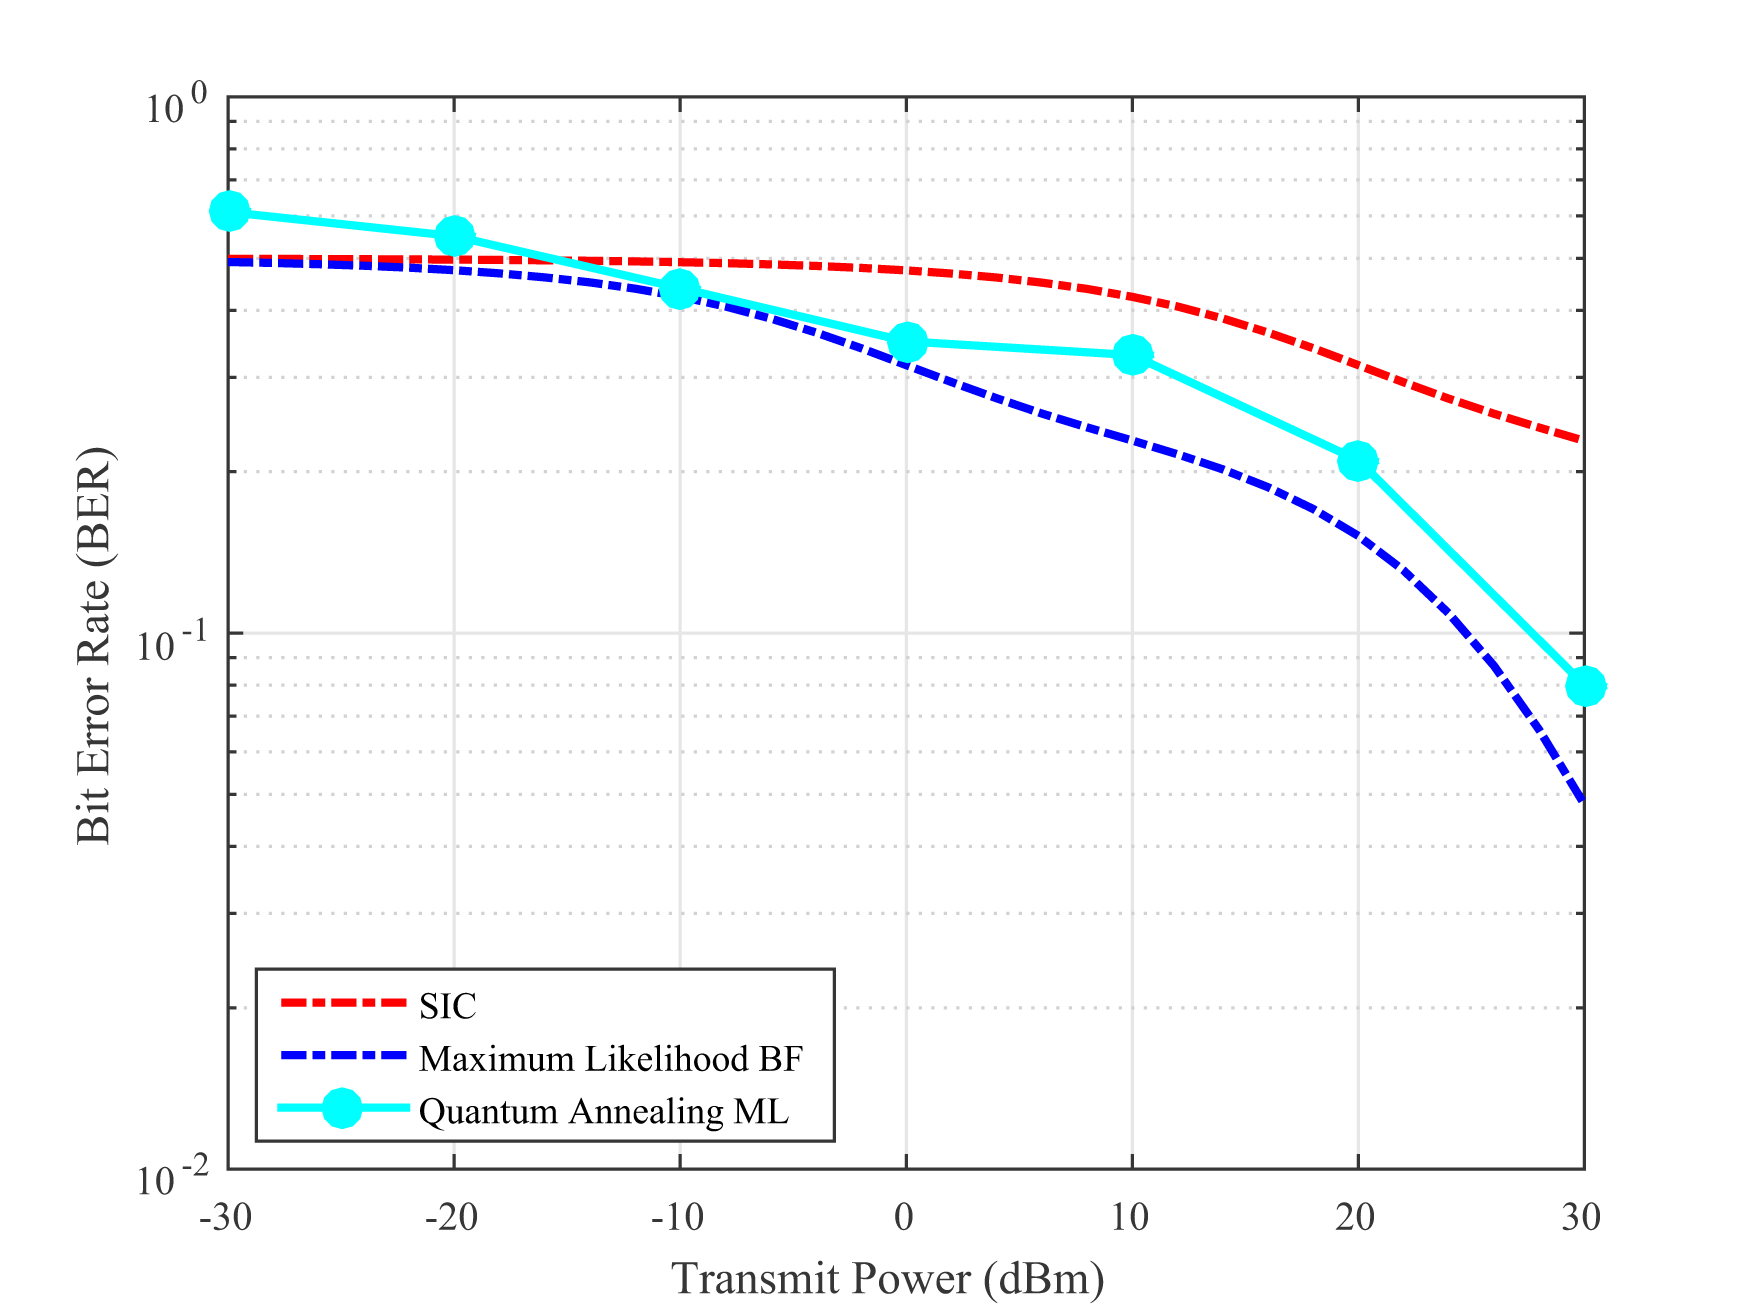
\includegraphics[width=0.85\linewidth]{Chapter3/Figs/16qamvs copy.png}
    \caption{The avergae BER performance vs. the transmit power for a 3 user NOMA scenario employing 16-QAM, with different decoding techniques.}
    \label{fig:16vs}
\end{figure}
At higher transmit power ML bruteforce solution clearly outperform both SIC and QA, although the gap between QA and ML is marginal.
similar to BPSK and QPSK, SIC curve enhances minimally until 15 dBm with the following saturation after this point.

Similarly, A thorough breakdown of the BER performance using the ML QA decoder with 16-QAM for users positioned at different cell locations is presented in \autoref{fig:16qam3}. the 3 users at diffrnet locations having different path loss experience almost the same BER until about 10 dbm. After that, the difference between them begins to grow considerably. The performance of the near user improves remarkably, where the middle user curve enhances minimally. The far user exhibit the same overall trend but has the worst performance of the 3. 


In general, the BER performance of QA maximum likelihood 16-QAM is comparable with the bruteforce solution.
\begin{figure}[H]
    \centering
    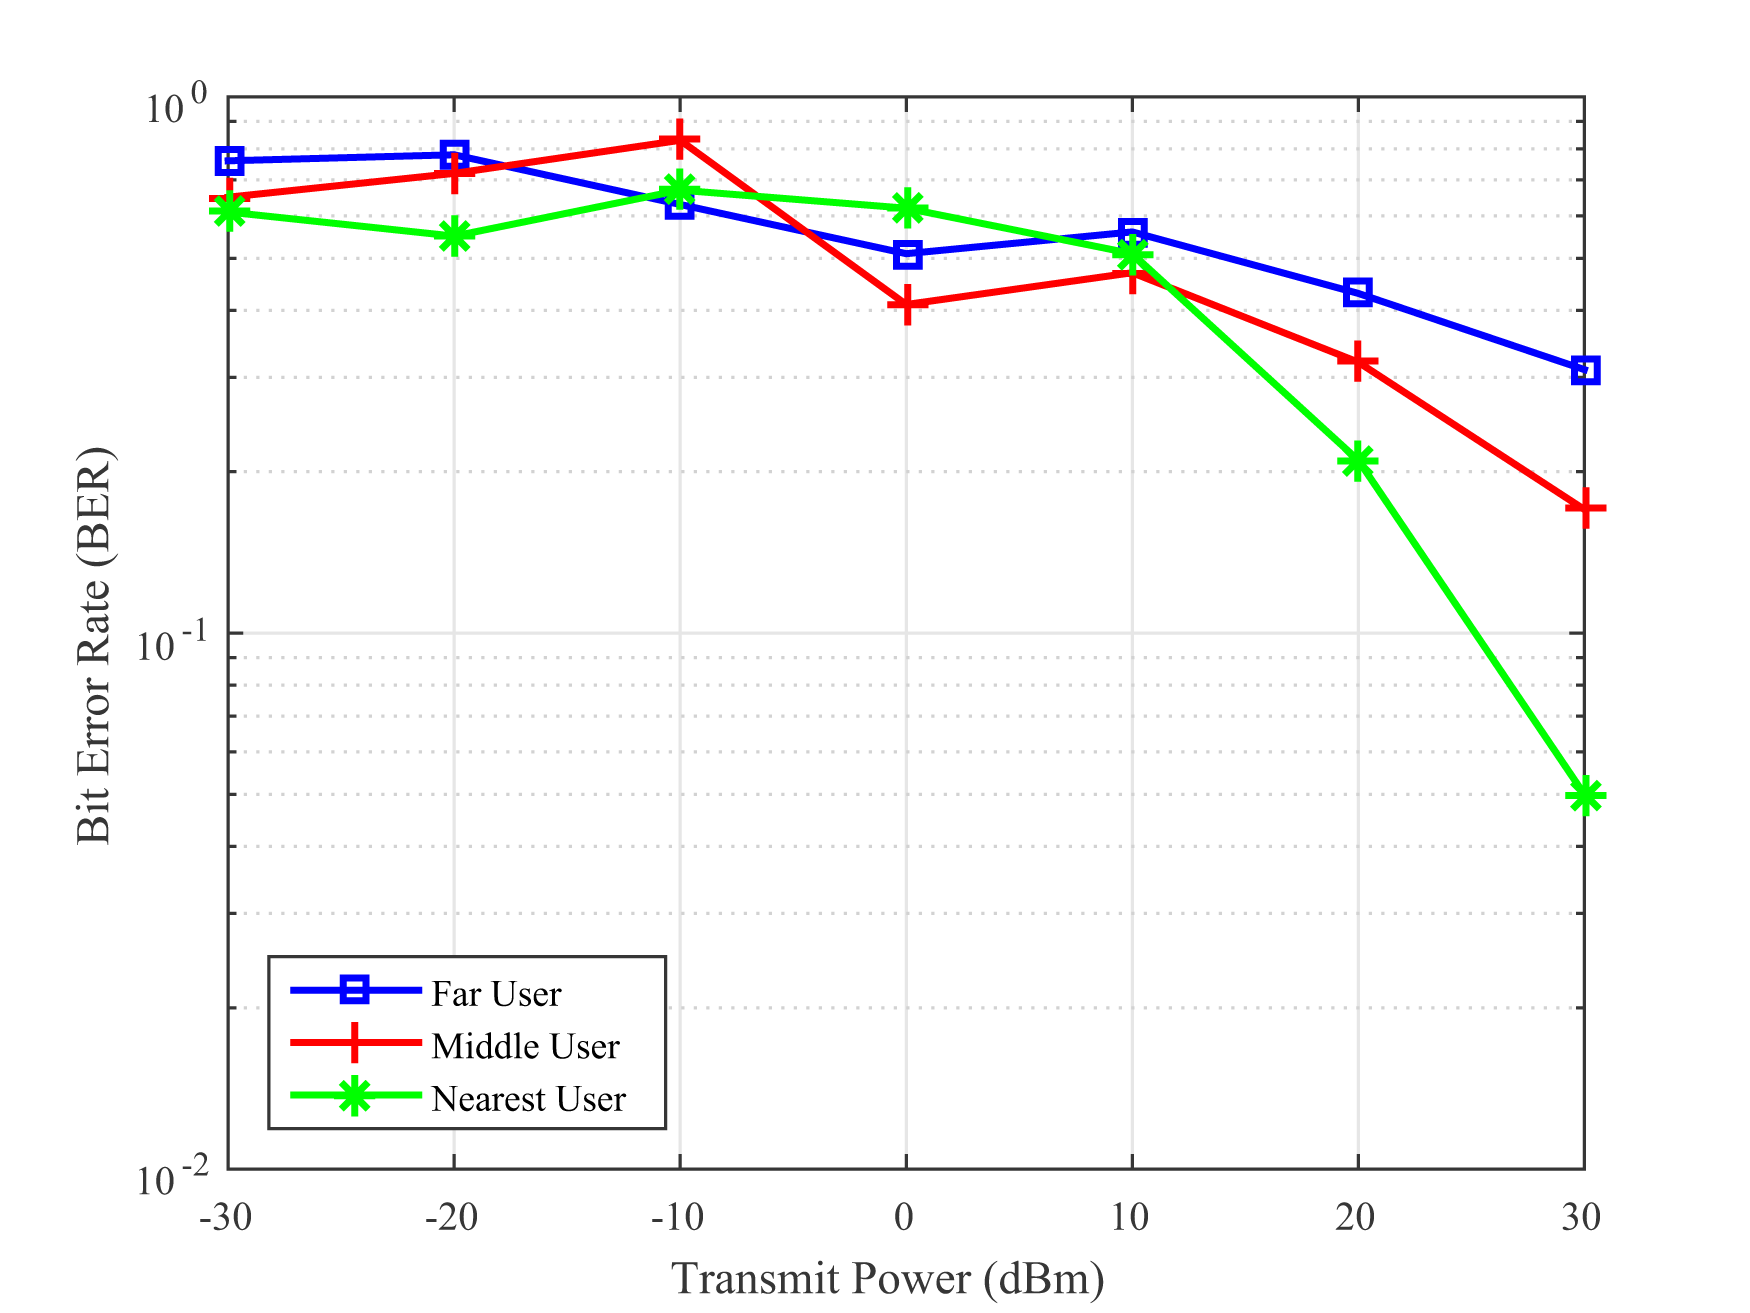
\includegraphics[width=0.85\linewidth]{Chapter3/Figs/16qam3 copy.png}
    \caption{The BER performance vs. the transmit power per user at different cell positions—near, middle, and far- for 16-QAM with Quantum Annealing based maximum likelihood decoder.}
    \label{fig:16qam3}
\end{figure}
\subsection{Bit-Error Rate Performance for QA Based Maximum-Likelihood detection with 64-QAM modulation}
In this study, we chose a scenario with only two users for the evaluation of 64-QAM modulation. This decision was based on the performance curve of the ML QA decoder versus the number of users, which indicated unacceptable BER levels for more than two users. Additionally, the brute force (BF) solution for ML detection in the case of 64-QAM is computationally intensive, as it must evaluate all possible symbols, resulting in considerably long processing times for high user count.

in \autoref{fig:64vs} First, we compared the three methods—BF, SIC, and QA—against each other. The results show a clear advantage of BF across the entire transmit power range.
\begin{figure}[H]
    \centering
    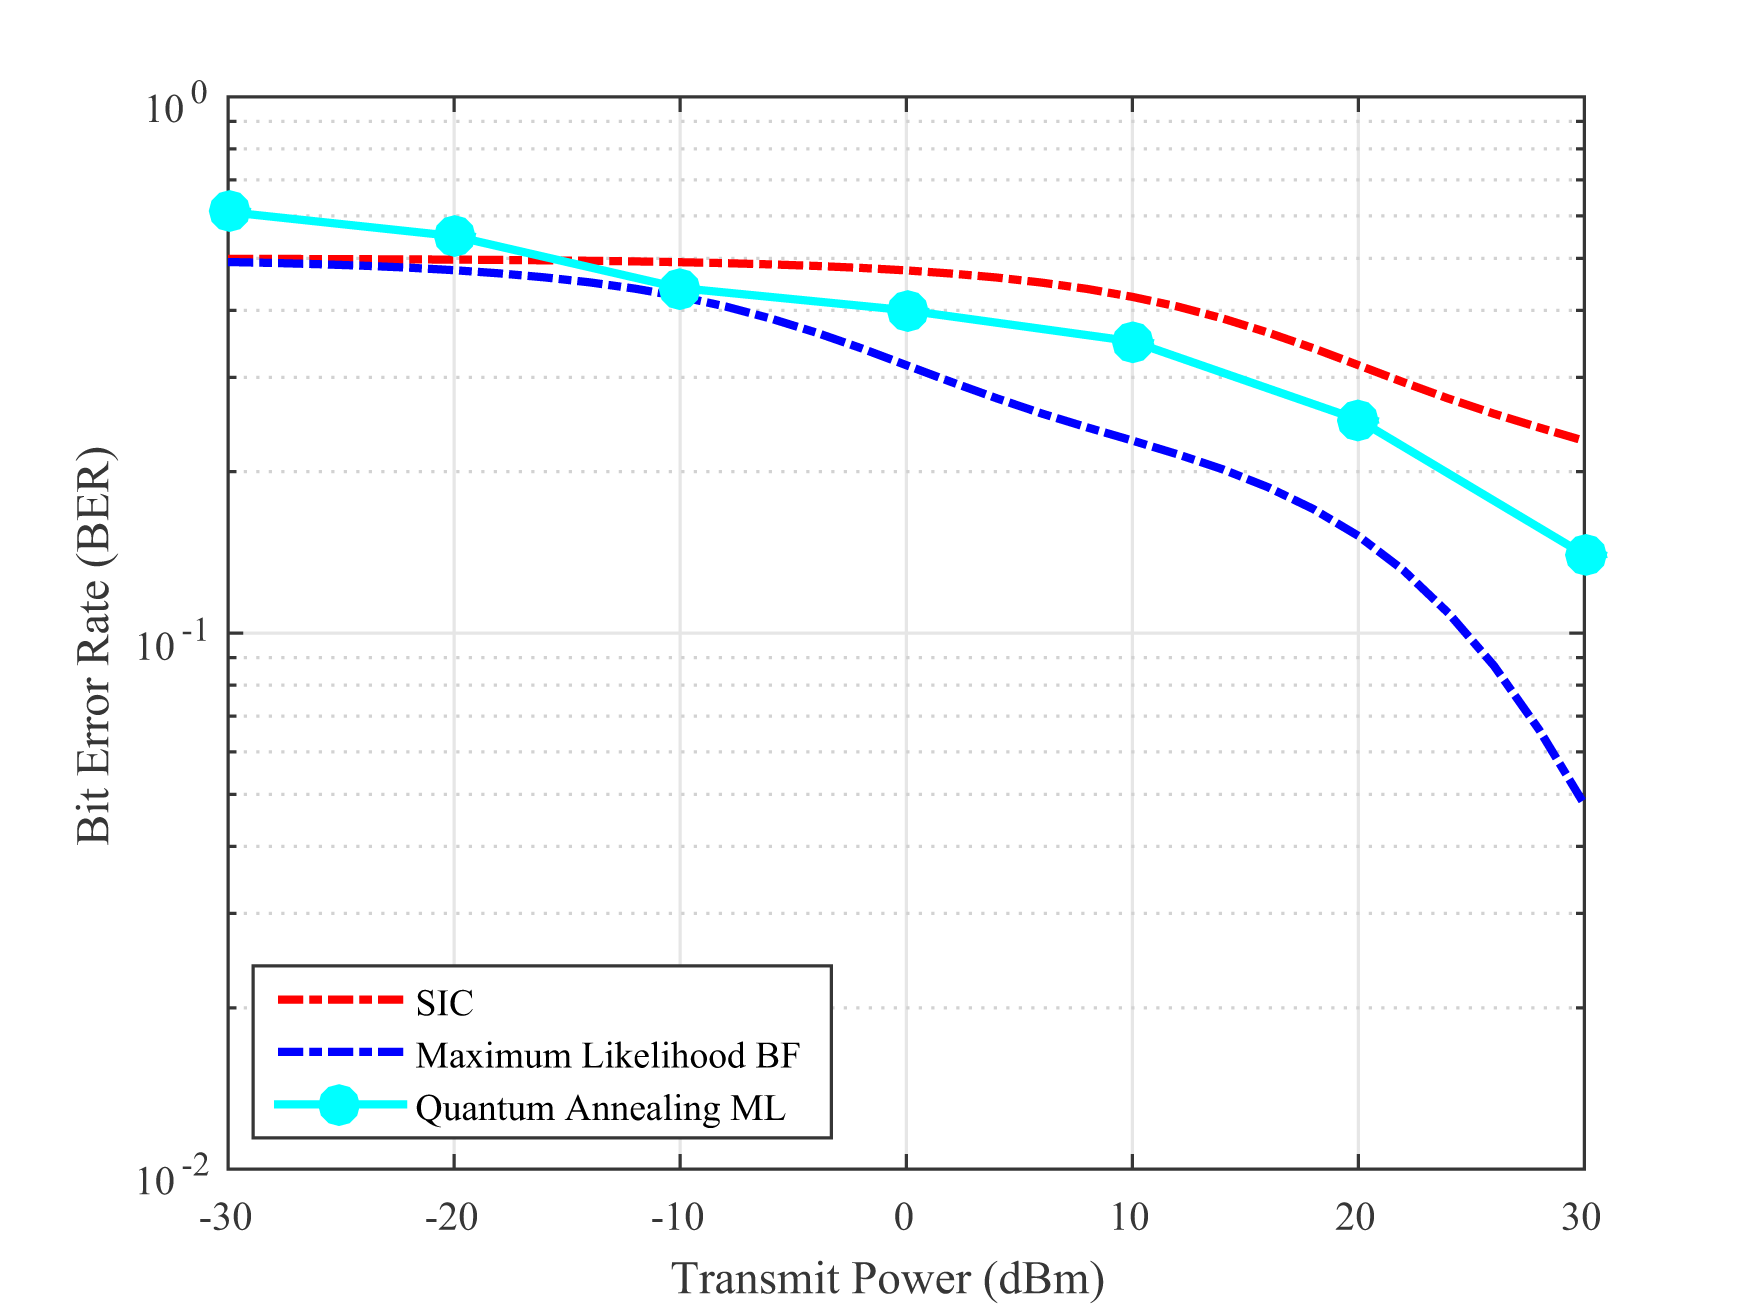
\includegraphics[width=0.85\linewidth]{Chapter3/Figs/64qamvs.png}
    \caption{The avergae BER performance vs. the transmit power for a 2 user NOMA scenario employing 64-QAM, with different decoding techniques.}
    \label{fig:64vs}
\end{figure}
BF consistently provides the lowest BER, demonstrating superior performance. In contrast, SIC suffers from performance degradation, delivering subpar results. Initially, QA exhibits a higher BER compared to the other methods. However, as the transmit power increases, QA's performance begins to improve. Although QA performs better than SIC, there remains a significant gap between QA and BF.


Unlike the previous analysis that averaged BER across users, in this evaluation, the BER of each user was assessed independently in \autoref{fig:64qam}. 
\begin{figure}[H]
    \centering
    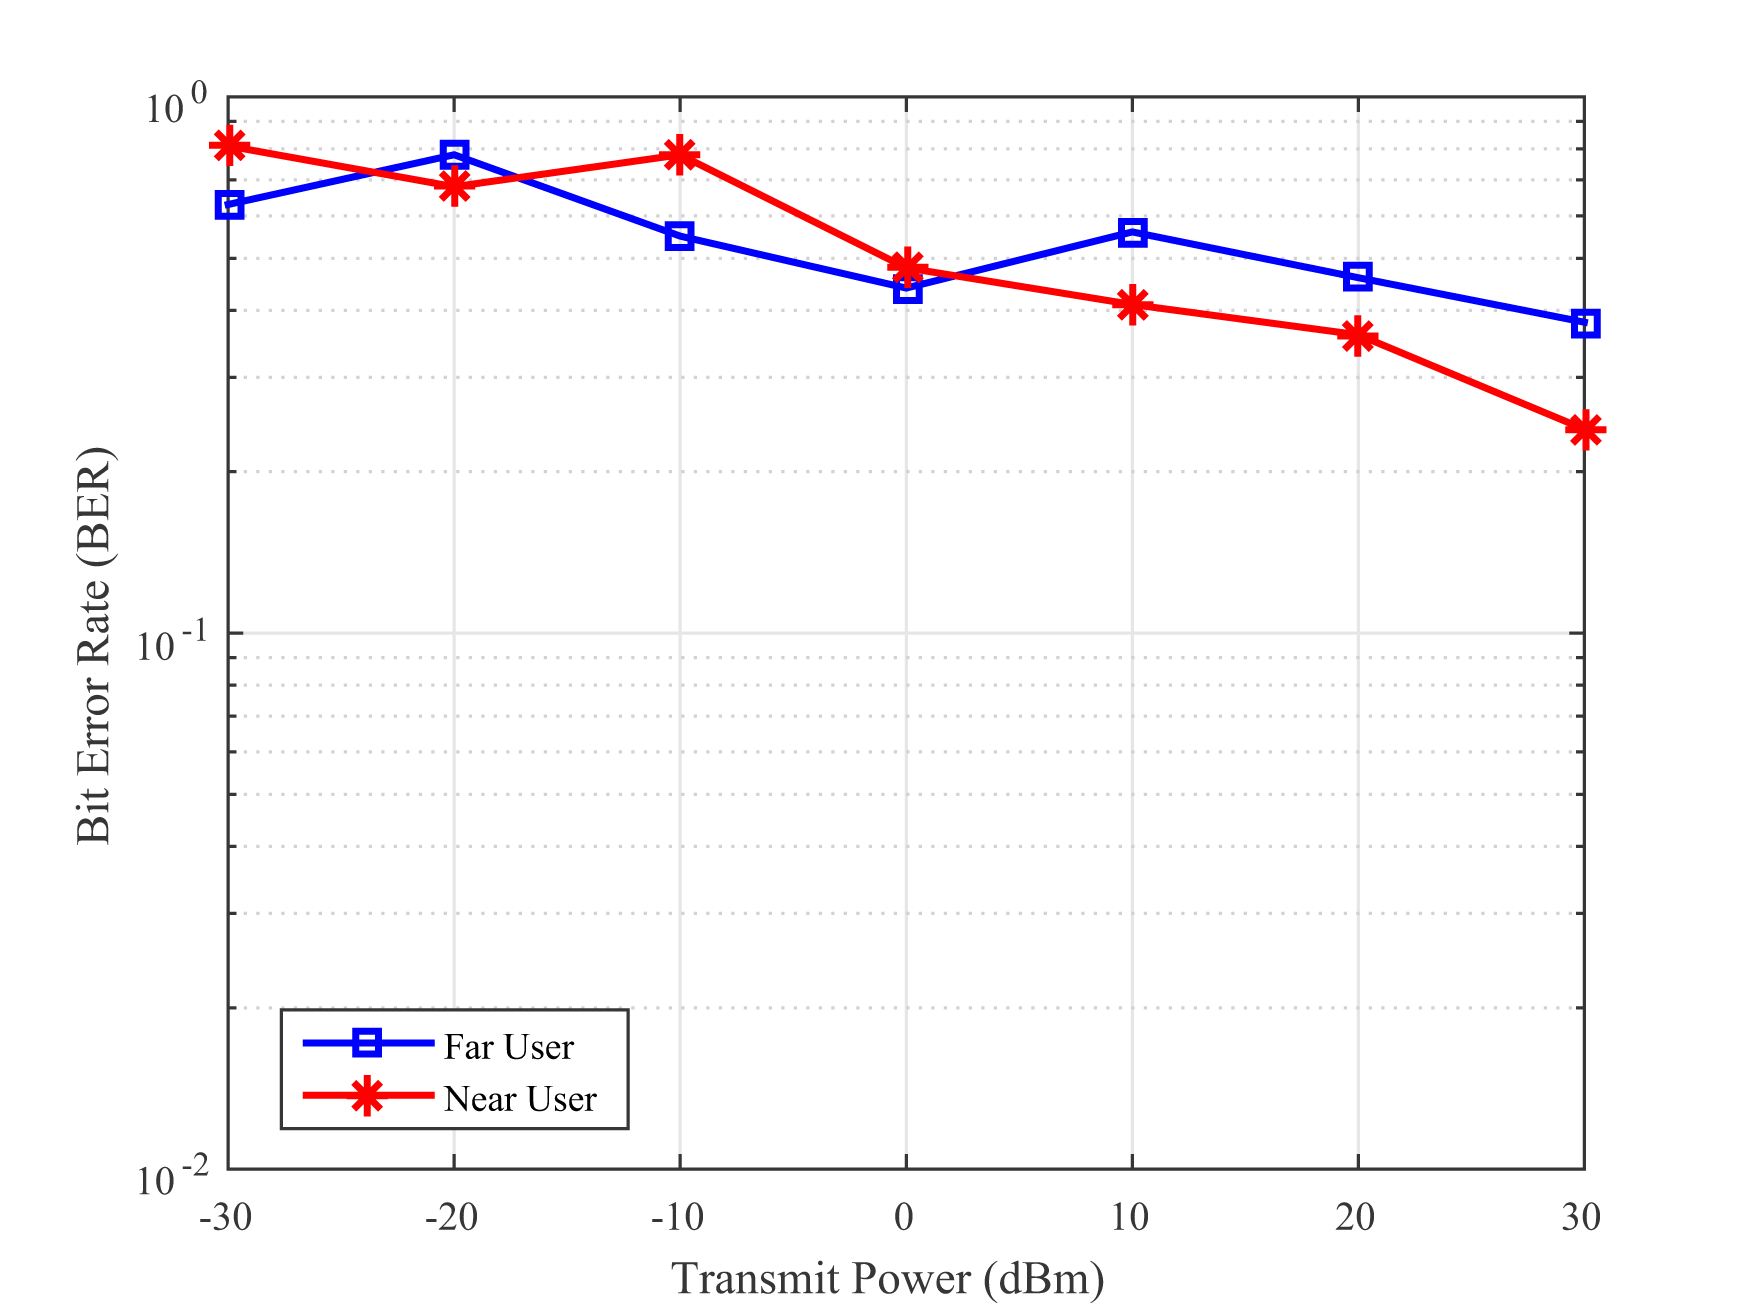
\includegraphics[width=0.85\linewidth]{Chapter3/Figs/64qam2 copy.png}
    \caption{The BER performance vs. the transmit power per user at different cell positions—near, and far- for 64-QAM with Quantum Annealing based maximum likelihood decoder.}
    \label{fig:64qam}
\end{figure}
The far user, positioned at 500 meters, and the near user, positioned at 100 meters, displayed mixed performance initially. Up to 0 dBm, the far user demonstrated slightly better or identical performance compared to the near user. However, beyond this point, the near user began to recover. The BER for the near user improved in a slow yet steady manner, ultimately providing better BER at higher transmit power levels.

In summary, QA shows promise by improving with increased power, while still lagging behind BF. SIC, on the other hand, fails to deliver competitive performance.

\paragraph{Note on BER Comparison between QA and BF:}
In the presented results, there are instances where QA shows a lower BER than ML bruteforce method for BPSK and QPSK due to different execution cycles, not superior performance. Specifically, QA was tested with fewer iterations and less frequent power steps (every 10 dBm), unlike BF, which used more bits and more frequent power steps (every 2 dBm). This led to BF's smoother curve compared to QA's more variable one.

With equal numbers of iterations and bit configurations, QA and BF results would converge, this is because both QA and BF are fundamentally based on the same Maximum Likelihood principle, and hence, under equivalent conditions, QA cannot outperform ML brute force in terms of BER.

\subsection{Comparison of Computation Time}
\label{subsec:execution_times}

\autoref{fig:time} illustrates the execution times for each decoding technique. The bar graph clearly shows that Successive Interference Cancellation (SIC) has the fastest execution time. The Brute Force (BF) method, involving iteration over all possible combinations, is the second fastest, as expected.
\vspace{-0.38cm}
\begin{figure}[H]
    \centering
    \includegraphics[width=0.76\linewidth]{timing copy1.png}
    \caption{Comparison between the decoding techniques in terms of simulation time for different modulations (in \textit{m}s).}
    \label{fig:time}
\end{figure}

The execution time for Quantum Annealing (QA) consists of several timing sub-intervals, such as programming time (\(T_p\)), annealing time (\(T_A\)), delay (\(T_D\)), and readout time (\(T_R\)), as detailed in \autoref{time}. While \(T_p\) and \(T_A\) are consistent across all cases, \(T_R\) and \(T_D\) vary slightly, depending on the number and position of physical qubits used—the more qubits, the longer the readout. The total post-processing time \(\Delta\) is minimal and generally negligible.

The brute-force solution for Maximum Likelihood (ML) decoding, requiring an exhaustive search, also demands substantial computation time. Though less time-consuming than QA, it remains computationally intensive, particularly with increasing numbers of users and modulation complexity.
SIC, by contrast, is notably faster. As it sequentially decodes and cancels the contributions of the strongest signals first, simplifying the decoding of subsequent signals. By avoiding exhaustive searches, SIC substantially cuts down computation time in NOMA systems compared to ML.

Overall, QA takes approximately twice the time of the SIC simulation, while BF is marginally faster than QA and comparable in speed. Notably, QA requires simulating the same problem \(R\) times (set to 1000 in this instance). However, parallelizing these simulations have shown significant reduce in overall QA simulation time compared to similar studies, suggesting a potential for efficiency improvements through parallel processing.

\textbf{Importantly, the true power of Quantum Annealing becomes evident when addressing large-scale problems, particularly those with high user counts and complex modulation schemes.} Although this aspect has not been empirically studied or simulated in this project, it is anticipated based on the computational requirements observed. Classical approaches, such as ML decoding, often become impractically complex and time-consuming under these conditions, typically rendering them unfeasible on classical computers. In contrast, QA is anticipated to efficiently manage such challenging scenarios. Table 4.1 provides an illustrative overview of potential user capacities for different modulation types, demonstrating QA's capability to support over 180 users in the BPSK case (\(2^{180} \approx 10^{54}\) possible symbols!), thereby making a strong case for its adoption in future communication systems where traditional methods are inadequate.





\chapter{Conclusion and Future Work}
\section{Conclusion}
NOMA has been widely recognized as a potential multiplexing scheme for next-generation networks due to its ability to improve spectrum efficiency. However, the implementation complexity of SIC receiver at the NOMA receiver has limited its full adoption in current 5G standards. As the number of users increases, SIC's latency and reliability performance deteriorates significantly. The error made in each iteration propagates through other successive iterations, and the power levels of each signal must be sufficiently different for successful detection. Various techniques such as user pairing/grouping, user scheduling, and multichannel transmission have been proposed to mitigate these issues. However, these approaches often consume additional network resources and somewhat contest the idea of transmission on overlapping resources on which the entire NOMA concept relies.

Maximum Likelihood (ML) detection is the optimal method for signal detection but is computationally heavy and often unfeasible on classical computers due to its NP-hard nature. In this project, we explored the QA-aided ML decoder for multi-user NOMA networks as an alternative to the SIC method. In our envisioned scenario, quantum processors will be co-located with C-RAN computational resources in a data center, partitioning the compute roles for hundreds of base stations or Remote Radio Heads (RRH) connected via low-latency optical fiber. Here, quantum computing will handle computationally demanding tasks.

Towards this objective, we first reformulated the signal estimation problem as a quadratic unconstrained binary optimization (QUBO) problem and ran it using D-Wave’s libraries on the newly released Advantage 5.2 QPU. We formulated the ML detection problem and derived the QUBO coefficients for different modulation schemes, including BPSK, QPSK, 16-QAM, and 64-QAM, enabling their solution using a QPU. To assess performance, we simulated a practical scenario involving a single base station, considering practical system parameters such as channel randomness and possible transmit power levels for all individual signals of all involved users.

In the obtained results, the QA-assisted ML decoder achieved similar Bit Error Rate (BER) performance as the brute force (BF) method and outperformed the SIC technique. Specifically, for BPSK and QPSK, the QA-aided decoder maintained low BER across various transmit power levels. For 16-QAM and 64-QAM, the QA-assisted decoder showed significant improvement in BER compared to SIC, but slightly higher BER compared to BF especially under higher modulation complexities. However, QA's execution time was longer than both BF and SIC. 

Even though the annealing time is in the order of microseconds, the total processing time for QA is much higher than classical computing due to the time required for sampling and readout. However, this can be enhanced as quantum engineering advances in superconducting qubit technology. Despite the relatively high programming time, QA presents an advantage over classical approaches for problems that are infeasible for the latter. QA does not require trying all possible cases to find the minimum distance solution.

\vspace{0.5cm}

Our performance results establish a baseline for future fully integrated systems within the context of the centralized RAN architecture. We show that once engineering efforts optimize the integration between quantum and conventional computation, quantum computation should be considered a competitive technology for the future design of high-capacity wireless networks.

\section{Future Work}


    
    \begin{itemize}
    \item In this project, the proposed method used forward annealing. Future work could employ reverse annealing to enhance solutions. Reverse annealing initiates from a programmable classical state, enabling a quasi-nonlocal search by increasing quantum fluctuations, which refine the search around the initial state. This method could synergize conventional classical detectors with quantum annealing-based detectors, allowing reverse annealing to probabilistically enhance initial solutions, akin to error correction using quantum effects.
    \item Exploration of more efficient embedding techniques, such as manual embedding, is recommended. Adjusting parameters like the number of reads, chain strength, and annealing time may better suit latency-sensitive tasks. Employing post-processing techniques, such as Single Qubit Correction (SQC), could also enhance results by iteratively optimizing each solution bit to lower Quantum Annealing energies.
    \item Investigating the use of gate-model quantum hardware for Maximum-Likelihood decoding is advised. Despite current devices' limitations in qubit numbers, future enhancements in quantum hardware might facilitate larger-scale experiments. Gate-model systems provide additional controls that could improve performance. Furthermore, exploring algorithms like the Quantum Approximate Optimization Algorithm (QAOA) and Grover's search algorithm may prove beneficial, despite the current qubit limitations.
    \item Future work should explore and compare hybrid, quantum-inspired, and classical solutions, such as D-Wave's Leap Hybrid service, which can handle up to 20,000 QUBO variables using problem partitioning. Other technologies like Coherent Ising Machines (CIM),\footnote{A CIM is a network of optical parametric oscillators (OPOs) programmed to solve Ising model-based problems, representing competitive interactions in magnetic systems.} digital annealing, and simulated annealing, offer potential quantum advantages on classical platforms, especially in environments where quantum hardware may not be available.
    \item Exploring the integration of NOMA with other wireless technologies—such as MIMO-NOMA, cooperative relaying, mmWave communications, beamforming, network coding, and advanced error correcting codes like LDPC and turbo codes—promises significant performance improvements and is a promising direction for future work.
    \item Upcoming investigations should consider the performance of QA-based ML detection in NOMA systems under imperfect channel state information (CSI) and challenging channel conditions, possibly modeled using ray tracing techniques.
    \item Future research should extend the application of QA to other NP-hard optimization problems in wireless communications, such as resource allocation, precoding, and scheduling.
\end{itemize}

    
    
    
    
    
    
    
    
    
    
   